\documentclass[12pt, a4paper, font, table]{article}
\usepackage[utf8]{inputenc}
\usepackage{amsmath}
\usepackage{commath}
\usepackage{amsfonts}
\usepackage{amssymb}
\usepackage{cancel}
\usepackage{graphicx}
\usepackage{titlesec}
\usepackage{multicol}
\usepackage[onehalfspacing]{setspace}
\usepackage{tikz}
\usepackage{ocgx2}
\usepackage{multicol}
\usepackage{enumitem}
\usetikzlibrary{positioning, fit, calc}
\tikzstyle{block} = [draw=black, thick, text width=.6cm, minimum height=.5cm, fill=blue!50]
\usepackage{xcolor, stackengine, pgffor}
\fontfamily{phvr}
\usepackage[left=3.00cm, right=2.00cm, top=3.00cm, bottom=2.00cm]{geometry}
\author{Tiago Menegaz}
\title{Matemática Básica}

\begin{document}
	
	%%% novoscomandos
	\renewcommand{\CancelColor}{\color{red}}
	%%% /novos comandos


\section{Regra dos sinais}
Demonstração da regra na adição e subtração

Por fazer\dots

\noindent Demonstração da regra na multiplicação e divisão

Imagine um retângulo com lados $6$ por $5$ que foi dividido em retângulos menores, com dimensão $ r1 = 1 X 3 $, outro com $ r2 = 5 X 3 $, outro com $ r3 = 1 X 2 $ e um com $ r4 = 5 X 2 $, assim: \\

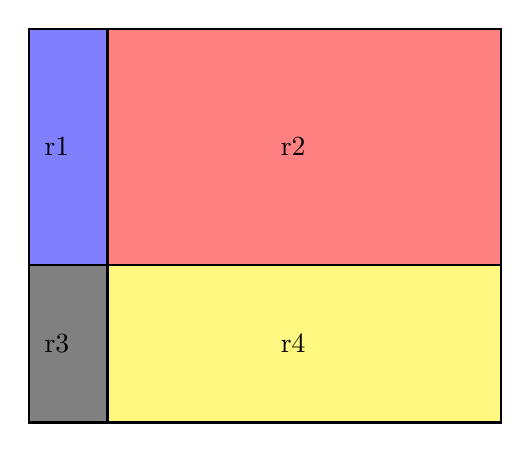
\begin{tikzpicture}
	\node[rectangle, draw,
	minimum width = 6cm,
	minimum height = 5cm,
	] (r) at (0,0) {6x5};

	\node[block,
	minimum width = 1cm,
	minimum height = 3cm
	] (r1) at ++(-2.5,1) {r1};

	\node[block, 
	fill=red!50,
	minimum width = 5cm,
	minimum height = 3cm
	] (r2) at ++(0.5,1) {r2};

	\node[block,
	fill=black!50,
	minimum width = 1cm,
	minimum height = 2cm
	] (r3) at ++(-2.5,-1.5) {r3};

	\node[block,
	fill=yellow!50,
	minimum width = 5cm,
	minimum height = 2cm
	] (r4) at ++(0.5,-1.5) {r4};
 \end{tikzpicture} \\

 Daí, sabe-se que a área de $ 6 X 5 = 1 \cdot 3 + 5 \cdot 3 + 1 \cdot 2 + 5 \cdot 2 $ \\
 $ \indent \indent \indent \indent \indent \indent \indent \indent \indent \; \: 30 = 3+15+2+10 $ \\
 $ \indent \indent \indent \indent \indent \indent \indent \indent \indent \; \: 30 = 30 $

 É então que, a partir dos valores obtidos do retângulo, podemos saber que para cada retângulo menor os valores são:

\begin{itemize}
	\item $ r1 = (6-5)(5-2) \Leftrightarrow r1 = 1 \cdot 3 $
	\item $ r2 = (6-1)(5-2) \Leftrightarrow r2 = 5 \cdot 3 $
	\item $ r3 = (6-5)(5-3) \Leftrightarrow r3 = 1 \cdot 2 $
	\item $ r4 = (6-1)(5-3) \Leftrightarrow r4 = 5 \cdot 2 $
\end{itemize}

Agora podemos montar uma expressão que melhor ilustre as equivalências e resolver: \\
$ (6-5)(5-2) + 5(5-2) + 1(5-3) + 5 \cdot 2 = 6X5 $ \\
$ (6-5)(5-2) + 25 - 10 + 5-3 + 5 \cdot 2 = 6X5 $ \\
$ 30 - 12 - 25 + 10 + 25 - 10 + 5-3 + 5 \cdot 2 = 6X5 $ \\
$ 30 - 12 \cancel{-25} \cancel{+10} \cancel{+25} \cancel{-10} + 5 - 3 + 5 \cdot 2 = 6X5 $ \\
$ 30 - 12 + 5 - 3 + 5 \cdot 2 = 6X5 $ \\
$ 20 + 5 \cdot 2 = 6 \cdot 5 \\
 \indent \! \! \! \! 20 + 10 = 6 \cdot 5 \\
 \indent \indent 30 = 30 $

\newpage

Isso quer dizer que se consideramos o maior valor de um lado como sendo $a$, menos o menor valor desse mesmo lado com $b$ e multiplicarmos pelo lado adjacente, que também tomou o maior como sendo $c$ e, então, subtrair do menor $d$, têm-se a equivalência: \\
 $ (a - b)(c - d) \Longrightarrow ac - ad - bc + bd$ \\

 Dá-se o nome a essa propriedade de \textbf{distributiva} do produto pela soma ou, nesse caso, pela diferença de dois números. \\
Como exemplo do produto pela soma, $ (a + b)(c + d) \Longrightarrow ac + ad + bc + bd$ \\

Outro exemplo para a mesma operação, só que desta vez com $3$ termos. \\
$ a(b+c) \Longrightarrow a \cdot b + a \cdot c $ 

\begin{itemize}
	\item $ 2(1 + 3) \Longrightarrow 2 \cdot 1 + 2 \cdot 3 = 8 $
\end{itemize}

Para as operações com números positivos o resultado é positivo. Na regra de sinais $ (+) \cdot (+) = (+) $. \\

Agora, para as operações que tem o produto de um número positivo por um número negativo, fica ssim:

\begin{itemize}
	\item $ 2(-5) \Longrightarrow 2 \cdot -5 = \;? $. Para resolver essa expressão deve ser considerada a aplicação da propriedade distributiva de tal modo que o resultado seja uma equivalência. É possível pensar que um equilíbrio pode ser obtido quando duas forças tendem a $0$, ou seja quando essa forças se anulam. Para isso o $2(-5)$ será zero se somente se $-5$ for somado ao $5$, daí para obter a igualdade deve ser feito o seguinte: \\ $ 2(+5 - 5) \Longrightarrow 2 \cdot 0 = 0 $
	\item por meio da distributiva, a soma dos $2$ produtos precisa ser entre opostos:\\ $ 2(+5-5) \Longleftrightarrow (2 \cdot +5) {\color{red}-} (2 \cdot {\color{red}+}5) \Longleftrightarrow +10 {\color{red}-} 10 = 0 $ 
\end{itemize}

Por meio das expressões apresentadas acima pode-se concluir que $ +a(-b) = -c $, ou seja, no produto pela diferença a regra de sinais é $(+) \cdot  (-) = (-) $. Isso também se aplica para $(-) \cdot  (+) = (-) $ por causa da propriedade comutativa \\

É possível adotar o mesmo pensamento para operaçõs do tipo $ (-a)(-b) $, contudo o resultado será $+c$.
Vejamos a seginte hipótese para a premissa:

\begin{itemize}
	\item $ (-3)(-4) = +c $ Para resolver presisamos de um número que somado a $(-4)$ ou a $(-3)$ o resultado seja $0$. Vou usar o $(+4)$ \\ $(-3)(-4+4) \Longrightarrow -3 \cdot 0 = 0$
	\item Com a distributiva a resolução da expressão fica assim: \\
	$ (-3)(-4+4) \\ ({\color{red}-} 3 ({\color{red}-} 4))+(-3 \cdot +4) $ \\
	$ \indent \; ({\color{red}+}12) \;\: + \; (-12) $ \\ $ \indent \indent +12 - 12 = 0 $
	\item portanto, podê-se concluir a partir da demostração de equivalência acima que \\ $ (-a)(-b) = (+c) $.
\end{itemize}

Para as operações de multiplicação entre número negativos o resultado é positivo. Na regra de sinais $ (-) \cdot (-) = (+) $. \\

A regra de sinais na multiplicação é, portanto a seguinte: 
 
 \begin{tabular}{|ccccc|}
	\hline
	(+) & $\cdot$ & (+) & $=$ & (+) \\
	\hline
	(+) & $\cdot$ & (-) & $=$ & (-) \\
	\hline
	(-) & $\cdot$ & (+) & $=$ & (-) \\
	\hline
	(-) & $\cdot$ & (-) & $=$ & (+) \\
	\hline
\end{tabular}


% \section{Potenciação}
Definição de potenciação:\\

$ a $ e $ m \in \mathbb{R} $ de tal forma que $ a^m = \mathbb{R}$.\\

Exemplos:

\begin{enumerate}[label=\alph*)]
\item $ a^{1} = a $
\item $ a^{0} = 1 $
\item $ 0^{0} = $ \textquestiondown (indeterminação) mas no assunto cálculo o $ 0^{0} = 1$
\item $ a^{m} = \underbrace{a \cdot a \cdot a \cdot a \ldots a}_{n\  fatores} $
\item $ 3 + 3 + 3 = 9 $
\item $ 3 \cdot 3 = 9 $
\item $ 3^{4} = 3\cdot 3\cdot 3\cdot 3 = 81 $
\item $ 3^{2} \cdot 3^{2} \Longrightarrow 3^{2+2} = 3^{4} $
\item $ 2^{2} + 2^{3} \Longrightarrow 1 \cdot 2^{2} + 2 \cdot 2^{2} \Longrightarrow 3 \cdot 2^{2} = 12 $
\item $ 4^{3} - 4^{2} \Longrightarrow 4^{1+2} - 4^{2} \Longrightarrow (4 \cdot 4^{2}) - 4^{2} \Longrightarrow 4^{2}(4 - 1) = 3 \cdot 4^{2} = 48 $
\item $ (-2)^{3} = (-2)\cdot (-2)\cdot (-2) = -8 $ (com expoente ímpar o resultado é negativo) 
\item $ (-2)^{4} = (-2)\cdot (-2)\cdot (-2)\cdot (-2) = 16 $
\item $ -2^{4} = -(2\cdot 2\cdot 2\cdot 2) = -16 $
\item $ 2^{3} + 3^{2} = 8 + 9 = 17 $
\item $ 2^{3} - 3^{2} = 8 - 9 = -1 $
\item $ 2^{3} + (-3)^{2} = 8 + 9 = 17 $
\item $ (-2)^{3} + 3^{2} = -8 + 9 = 1 $
\item $ -2^{3} - (-3)^{2} = -8 - 9 = -17 $
\item $ 2^{3} \cdot 3^{2} = 8 \cdot 9 = 72 $
\item $ \dfrac{3^{2}}{2^{3}} = 3^{2}\cdot \dfrac{1}{2^{3}} \longrightarrow 9 \cdot \dfrac{1}{8} = \dfrac{9}{8}$
\end{enumerate}

\subsection{Propriedades da potenciação}
\begin{enumerate}[label=P\roman*)]
	\item $ a^{m} \cdot a^{n} = a^{m+n} \longrightarrow 2^{3} \cdot 2^{2} = 2^{3+2} = 2^{5} = 32 $
	\item $ (a^{m})^{n} = a^{m\cdot n} \longrightarrow (2^{3})^{2} = 2^{3}\cdot 2^{3} = 2^{3+3} $ ou $ 2^{3\cdot 2} = 2^{6} = 64 $
	\item $ a^{-m} = \dfrac{1}{a^{m}}\ (OBS: a \neq 0)$
	\begin{enumerate}[label=\alph*)]
		\item $ 3^{-2} = \dfrac{1}{3^{2}} = \dfrac{1}{9}; $
		
		\item $\dfrac{1}{2^{-3}} = 2^{3} = 8 $ 
	\end{enumerate}
	\item $ \dfrac{a^{m}}{a^{n}} = a^{m-n} \longrightarrow \dfrac{3^{5}}{3^{2}} = 3^{5}\cdot \dfrac{1}{3^{2}} \longrightarrow 3^{5}\cdot 3^{-2} = 3^{5+(-2)} = 3^{3} = 27$
	\item $ a^{m}\cdot b^{m}= (a\cdot b)^{m} \longrightarrow 2^{3}\cdot 3^{3} = (2\cdot 3)^{3} = 6^{3} = 216 $
	\item $ \dfrac{a^{m}}{b^{m}} = (\dfrac{b}{a})^{m} \longrightarrow (\dfrac{8^{3}}{2^{3}}) = (\dfrac{8}{2})^{3} = 4^{3} = 64 $
	\item $ (\dfrac{a}{b})^{-m} = (\dfrac{b}{a})^{m} $ (OBS: deriva das $ Piii $ e $ Piv $)
	\begin{enumerate}[label=\alph*)]
		\item $ (\dfrac{3}{2})^{-3} = \dfrac{3^{-3}}{2^{-3}} \Longrightarrow \dfrac{1}{3^{3}}\cdot \dfrac{1}{2^{-3}} \Longrightarrow \dfrac{1}{3^{3}}\cdot \dfrac{2^{3}}{1} \Longrightarrow \dfrac{2^{3}}{3^{3}} = (\dfrac{2}{3})^{3} $
		
		\item $ (\dfrac{2}{4})^{-3} = \dfrac{2^{-3}}{4^{-3}} \Longrightarrow \dfrac{4^{3}}{2^{3}} = (\dfrac{4}{2})^{3}  = 2^{3} = 8 $
		
		\item $ (5 \div 3)^{-2} = (\dfrac{5}{1} \cdot \dfrac{1}{3})^{-2} \Longrightarrow (\dfrac{1}{5} \cdot \dfrac{3}{1})^{2} = (\dfrac{3}{5})^{2} $
		
		\item $ (12 \div 6)^{-2} = (\dfrac{2}{1})^{-2} \Longrightarrow (\dfrac{1}{2})^{2} $
	\end{enumerate}
\end{enumerate}

\subsection{Questões}
\begin{enumerate}[label=\alph*)]
	\item Sendo $ x $ e $ y $ números reais não nulos, a expressão $ (x^{-2} + y^{-2})^{-1} $ é o mesmo que:

	\indent \indent \textbf{Resposta}:
	
	\indent \indent $ (\dfrac{1}{x^{2}} + \dfrac{1}{y^{2}})^{-1} \Longrightarrow (\dfrac{y^{2} + x^{2}}{x^{2}\cdot y^{2}})^{-1} \Longrightarrow \dfrac{x^{2} \cdot y^{2}}{y^{2} + x^{2}} = \dfrac{(x \cdot y)^{2}}{y^{2} + x^{2}} $
	
	\item A fração $ \dfrac{2^{98} + 4^{50} - 8^{34}}{2^{99} - 32^{20} + 2^{101}} $ é igual a qual fração?
	
	\indent \indent \textbf{Resposta}:
	
	\indent \indent $ \dfrac{2^{98}}{2^{99}} = 2^{98 - 99} = 2^{-1} = \dfrac{1}{2} $ \\

	\indent \indent $ \dfrac{4^{50}}{-32^{20}} \Longrightarrow \dfrac{4^{50}}{-(8\cdot 4)^{20}} \Longrightarrow \dfrac{(2^{2})^{50}}{-(2^{3}\cdot 2^{2})^{20}} \Longrightarrow \dfrac{2^{2\cdot 50}}{-(2^{3 + 2})^{20}} \Longrightarrow \dfrac{2^{100}}{-(2^{5\cdot 20})} = \dfrac{2^{100}}{-2^{100}} $ \\
	
	\indent \indent $ \dfrac{-8^{34}}{2^{101}} \Longrightarrow \dfrac{-(2^{3})^{34}}{2^{101}} \Longrightarrow \dfrac{-2^{3\cdot 34}}{2^{101}} \Longrightarrow \dfrac{-2^{102}}{2^{101}} $ \\
	
	\indent \indent $ \dfrac{2^{98} + 2^{100} - 2^{102}}{2^{99} - 2^{100} + 2^{101}} \Longrightarrow \dfrac{2^{98}(1 + 2^{2} - 2^{4})}{2^{99}(1 - 2^{1} + 2^{2})} \Longrightarrow \dfrac{1(1 + 4 - 16)}{2(1 - 2 + 4)} \Longrightarrow \dfrac{1 \cdot -11}{2\cdot 3} = \dfrac{-11}{6}  $
	
	\item O valor de $ 0,2^{3} \cdot 1,6^{2} $ é:
	
	\indent \indent \textbf{Resposta}:

	\indent \indent $ \dfrac{2}{10}^{3} \cdot \dfrac{16}{10}^{2} \Longrightarrow \dfrac{2}{10}^{3} \cdot ((\dfrac{2}{10}^{2})^{2})^{2} \Longrightarrow \dfrac{2}{10}^{3+8} = \dfrac{2}{10}^{11} $ 
	
	\item Encontre a solução para a expressão numérica $ \dfrac{4^{2} + (5 - 3)^{2}}{(9 - 7)^{2}} $
	
	\indent \indent \textbf{Resposta}:
	
	\indent \indent $ \dfrac{(2^{2})^{2} + 2 ^{2}}{2^{2}} \Longrightarrow \dfrac{\cancel{2^{2}}(2^{2} + 1)}{\cancel{2^{2}}} \Longrightarrow 4 + 1 = 5 $

\end{enumerate}
	
	\textbf{Reduza a uma potência}
\begin{enumerate}[label=\alph*)]
	
	\item $ (-2^{2})^{2} $
	
	\indent \indent \textbf{Resposta}: $ (-2^{2})(-2^{2}) \Longrightarrow 2^{2+2} = 2^{4} $\\
	
	\item $ \dfrac{4}{8} $
	
	\indent \indent \textbf{Resposta}: $ \dfrac{2^{2}}{2^{3}} \Longrightarrow 2^{2-3} = 2^{-1} $\\
	
	\item $ 5^{2}\cdot 5^{5}\cdot 5^{-1} $
	
	\indent \indent \textbf{Resposta}: $ 5^{2+5} \cdot \dfrac{1}{5} \Longrightarrow 5^{7} \cdot \dfrac{1}{5} \Longrightarrow \dfrac{5^{7}}{5} \Longrightarrow 5^{7-1} = 5^{6} $ \\	
	
	\item $ \dfrac{3^{6}\cdot 3^{-2}}{3^{4}} $
	
	\indent \indent \textbf{Resposta}: $ \dfrac{3^{6-2}}{3^{4}} \Longrightarrow 3^{6 - 2}\cdot 3^{-4} \Longrightarrow 3^{6-2-4} = 3^{0} = 1 $ \\
	
	\item $ \sqrt[4]{\dfrac{2^{65}+2^{67}}{10}} $
	
	\indent \indent \textbf{Resposta}: $ \sqrt[4]{\dfrac{2^{65}+2^{65}\cdot 2^{2}}{10}} \Longrightarrow \sqrt[4]{\dfrac{(1+4)2^{65}}{10}} \Longrightarrow \sqrt[4]{\dfrac{2^{65}\cdot 5}{2\cdot 5}} \Longrightarrow \sqrt[4]{\dfrac{2^{65}\cdot \cancel{5}}{2\cdot \cancel{5}}} \Longrightarrow \sqrt[4]{2^{65-1}} \Longrightarrow \sqrt[4]{2^{64}} = 2^{16} $
	

\end{enumerate}

% 	
 \section{Introdução a fração}
 	Sendo \textbf{a} e \textbf{b} números pertencentes a \textbf{$\aleph$} com \textbf{b} diferente de \textbf{0}, tem-se que $\dfrac{\textbf{a}}{\textbf{b}}$  (significa \textbf{a} dividido por \textbf{b}, ou simplesmente \textbf{a} $\div$ \textbf{b}), será um número \textbf{$\aleph$} se e somente se \textbf{a} for múltiplo de \textbf{b}. Em sendo diferente, a relação de \textbf{a} dividido por \textbf{b}, o número poderá ser \textbf{$\Re$}
 	
 	Então chamamos de $\dfrac{\textbf{a}}{\textbf{b}}$ de fração onde \textbf{a} é o numerador e \textbf{b} é o denominador. Nem sempre $\dfrac{\textbf{a}}{\textbf{b}}$ será um número natural pois a \textbf{ideia da fração é dividir em partes iguais} e dentre estas partes, consideraremos \textbf{umas} ou \textbf{algumas}, conforme o nosso interesse.
 	
 	As frações podem ser classificadas da seguinte forma, a saber:\\
 	
 	\indent \indent Fração \textbf{própria}: numerador $<$ denominador: $\dfrac{\textbf{2}}{\textbf{3}}$, $\dfrac{\textbf{1}}{\textbf{4}}$, $\dfrac{\textbf{3}}{\textbf{5}}$ \\
 	
 	\indent \indent Fração \textbf{imprópria}: numerador $\ge$ denominador: $\dfrac{\textbf{4}}{\textbf{3}}$, $\dfrac{\textbf{6}}{\textbf{5}}$, $\dfrac{\textbf{8}}{\textbf{5}}$ \\
 	
 	\indent \indent Fração \textbf{mista}: numerador $\geq$ denominador. Considerando-se duas frações: $\dfrac{\textbf{3}}{\textbf{3}}$ + $\dfrac{\textbf{4}}{\textbf{3}}$ é o mesmo que $ 1 + \dfrac{4}{3} $, onde o $ 1 $ é a simplificação de $\dfrac{\textbf{3}}{\textbf{3}}$. Tendo em vista outra fração mista, a foma de escreve pode ser apresentada assim: $\textbf{3}\dfrac{\textbf{4}}{\textbf{2}}$, ou, de forma detalhada:\\
 	
 	$\dfrac{\textbf{2}}{\textbf{2}} + \dfrac{\textbf{2}}{\textbf{2}} + \dfrac{\textbf{2}}{\textbf{2}} + \dfrac{\textbf{4}}{\textbf{2}} = \dfrac{\textbf{10}}{\textbf{2}}$. \\
 	
 	Observe que existe uma soma de frações com bases iguais e que, portanto, basta multiplicar o inteiro pelo denominador e somar ao numerador, preservando a base. \\
 	Ou seja, para $ 2\dfrac{3}{5} $ têm-se $ 5 \cdot 2 + 3 = 13 \longrightarrow \dfrac{13}{5} $. 
	Isso quer dizer que a fração $\dfrac{\textbf{5}}{\textbf{5}}$ será somada a $\dfrac{\textbf{5}}{\textbf{5}}$ e, em seguida, adicionada a fração $\dfrac{\textbf{3}}{\textbf{5}}$.
 	
 	O processo inverso é feito pela divisão da fração imprópria. Para transformar $ \dfrac{23}{6} $ em fração mista, faz-se assim: \\
 	
 	\begin{multicols}{2}[de fração imprópria $ \longrightarrow $ para fração mista]
	\setlength{\columnseprule}{.5pt}
 	$
 	\begin{array}{l l r r}
 	\multicolumn{2}{r}{23} \vline & \multicolumn{2}{c}{6} \\ \cline{3-4}
 	\multicolumn{2}{l}{-18} & \multicolumn{2}{l}{\color{red}3} \\ \cline{1-2}
 	\multicolumn{2}{r}{\color{blue}5} &  \\
 	\end{array}
 	$ 	
	\hrule
 	\columnbreak
	$
	\color{red}3 \dfrac{\color{blue}5}{\color{black}6} \color{black} \longrightarrow \color{red}3 \cdot \color{black}6 + \color{blue}5 = \color{black}23 \longrightarrow \dfrac{23}{6}
	$
	\newline
	\newline
	\hrule 
 \end{multicols}


\indent Fração \textbf{aparente}: numerador é múltiplo do denominador: $\dfrac{\textbf{4}}{\textbf{2}}$, $\dfrac{\textbf{6}}{\textbf{2}}$, $\dfrac{\textbf{24}}{\textbf{12}}$ \\
	 	
 	As \textbf{Frações Equivalentes} são frações que representam a mesma parte do todo. Veja que as frações $\dfrac{\textbf{1}}{\textbf{2}}$, $\dfrac{\textbf{2}}{\textbf{4}}$ e $\dfrac{\textbf{4}}{\textbf{8}}$, são equivalentes, pois multiplicando o numerador e o denominador por um número \textbf{$\aleph \neq 0$} tem-se o seu equivalente. Tomemos como exemplo a fração $\dfrac{\textbf{1}}{\textbf{2}}$ que tem o seu numerador e seu denominador multiplicados por $\textbf{2, 3, 4}$ e $\textbf{5}$: \\
 	
 	$\dfrac{1\cdot\textbf{2}}{2\cdot\textbf{2}} = \dfrac{2}{4} \longrightarrow \dfrac{1\cdot\textbf{3}}{2\cdot\textbf{3}} = \dfrac{3}{6} \longrightarrow \dfrac{1\cdot\textbf{4}}{2\cdot\textbf{4}} = \dfrac{4}{8} \longrightarrow \dfrac{1\cdot\textbf{5}}{2\cdot\textbf{5}} = \dfrac{5}{10}$ \\
 	
 	Conhecer as frações equivalente é importante para executar o processo de \textbf{simplificação de frações} até a obtenção de seu termo \textbf{irredutível}. Vajamos a fração $\dfrac{9}{12}$. O fator comum para $9$ e $12$ é o $\textbf{3}$. Então $\dfrac{9\div\textbf{3}}{12\div\textbf{3}} = \dfrac{3}{4}$ que é a fração irredutível (não possui fator comum). \\
 	
 	A partir do entendimento de frações equivalente podemos trabalhar com o número fracionário: $\dfrac{\textbf{m}}{\textbf{n}}$ com $\textbf{n} \neq \textbf{0}$ e $\dfrac{\textbf{m}}{\textbf{n}} \neq \aleph $. \\
 	
 	\noindent Então, para $\textbf{5}\cdot \textbf{x} = 1$ devemos pensar qual o valor de \textbf{x} para que o resultado da multiplicação por \textbf{5} seja \textbf{1}? Fica claro que \textbf{x} não pode ser um numero $\aleph $. Por isso devemos usar um \textbf{número fracionário}, qual seja $\dfrac{1}{5}$, pois $\textbf{5}\cdot \dfrac{\textbf{1}}{\textbf{5}} = \dfrac{\textbf{5}}{\textbf{5}} = 1$.
 	
 
 \subsection{Exemplo}
 \begin{enumerate}
 	
 	\item Na fração $\dfrac{\textbf{8}}{\textbf{2}}$ obtemos o quociente 4, então $\dfrac{\textbf{a}}{\textbf{b}}$ é um número natural e \textbf{8} é múltiplo de \textbf{2}. É uma fração \textbf{aparente}
 	
 	\item Raquel comeu $\dfrac{\textbf{3}}{\textbf{4}}$ de uma barra de chocolate. Isso significa que se dividirmos a barra em \textbf{4} partes iguais Raquel teria comido \textbf{3} partes e apenas uma teria sobrado.  É uma fração \textbf{própria}
 
 	\item Considere o retângulo
 		
 		\begin{tabular}{|c|c|c|c|}
 			\hline
 			\cellcolor{blue} & \cellcolor{blue} & & \cellcolor{blue} \\
 			\hline
 			& \cellcolor{blue} & \cellcolor{blue} & \\
			\hline
 		\end{tabular}
 	
 	\begin{enumerate}[label=\alph*)]
	 	\item Em quantas partes iguais o retângulo foi dividido?  dividido em $\textbf{8}$ partes.
	 	\item Cada uma destas partes representa que fração do retângulo?  $\space$ representa $\space \dfrac{\textbf{1}}{\textbf{8}}$
	 	\item A parte pintada representa que fração do retângulo? $\space$ representa $\space \dfrac{\textbf{5}}{\textbf{8}}$
	\end{enumerate}
		
 		\item Observe os retângulos abaixo e diga quanto representa cada parte da figura e a parte pintada
 		
 		\begin{enumerate}[label=\alph*)]
 		\item \begin{tabular}{|c|c|c|c|}
 			\hline
 			\cellcolor{yellow} & \cellcolor{yellow} & \cellcolor{yellow} & \cellcolor{yellow} \\
 			\hline
 			& \cellcolor{yellow} & \cellcolor{yellow} & \\
 			\hline
 			\cellcolor{yellow} & \cellcolor{yellow} & &\cellcolor{yellow} \\
 			\hline
 		\end{tabular}	
 	representa $\space \dfrac{\textbf{1}}{\textbf{12}}$ e a parte pintada $\space$ representa $\space \dfrac{\textbf{9}}{\textbf{12}}$
	 	
	 	\item \begin{tabular}{|c|c|c|}
	 		\hline
	 		\cellcolor{gray} & \cellcolor{gray} & \cellcolor{gray} \\
	 		\hline
	 		& \cellcolor{gray} & \cellcolor{gray} \\
	 		\hline
	 	\end{tabular}
	 	representa $\space \dfrac{\textbf{1}}{\textbf{6}}$ e a parte pintada $\space$ representa $\space \dfrac{\textbf{5}}{\textbf{6}}$
		
	\item \begin{tabular}{|c|c|}
		\hline
		\cellcolor{green} & \cellcolor{green} \\
		\hline
		\cellcolor{green} & \cellcolor{green} \\
		\hline
	\end{tabular}
representa $\space \dfrac{\textbf{1}}{\textbf{4}}$ e a parte pintada $\space$ representa $\space \dfrac{\textbf{4}}{\textbf{4}}$
	\end{enumerate}
	
	\item Para $\dfrac{\textbf{1}}{\textbf{6}}$ de uma pizza o custo é R\$$3,00$, quanto custa: \\
	
		\begin{enumerate}[label=\alph*)]
			\item $\dfrac{\textbf{3}}{\textbf{6}}$ da pizza? Custa R\$$9,00$ pois $\dfrac{\textbf{1}}{\textbf{6}} + \dfrac{\textbf{1}}{\textbf{6}} + \dfrac{\textbf{1}}{\textbf{6}} = \dfrac{\textbf{3}}{\textbf{6}}$ \\ \newline $\therefore 3,00 + 3,00 + 3,00 = 9,00$ ou ainda $3^{2}$ \\
			
			\item $\dfrac{\textbf{5}}{\textbf{6}}$ da pizza? Custa R\$$15,00$ pois $\dfrac{\textbf{1}}{\textbf{6}} + \dfrac{\textbf{1}}{\textbf{6}} + \dfrac{\textbf{1}}{\textbf{6}} + \dfrac{\textbf{1}}{\textbf{6}} + \dfrac{\textbf{1}}{\textbf{6}} = \dfrac{\textbf{5}}{\textbf{6}}$ \\ \newline $\therefore 3,00 + 3,00 + 3,00 + 3,00 + 3,00 = 15,00$ ou ainda $3\cdot5$ \\
			
			\item A pizza toda? Custa R\$$18,00$ ou ainda $3 \cdot 6$
		\end{enumerate}
	
	\item Se $\dfrac{\textbf{3}}{\textbf{7}}$ do que eu tenho são R\$$195,00$, a quanto corresponde $\dfrac{\textbf{4}}{\textbf{5}}$ do que eu tenho? \\ Cada parte do todo é representado por $\dfrac{\textbf{1}}{\textbf{7}} \Rightarrow \dfrac{\textbf{1}}{\textbf{7}} + \dfrac{\textbf{1}}{\textbf{7}} + \dfrac{\textbf{1}}{\textbf{7}} = \dfrac{\textbf{3}}{\textbf{7}}$ que então pode ser encontrada com $\dfrac{\textbf{195,00}}{\textbf{3}} \therefore \dfrac{\textbf{1}}{\textbf{7}} = 65$. \\
	Agora para saber quanto eu tenho: $\textbf{65,00}\cdot\textbf{7} \therefore \dfrac{\textbf{7}}{\textbf{7}} = 445$. \\
	O próximo passo é saber quanto são $\dfrac{\textbf{4}}{\textbf{5}}$ do que eu tenho (R\$$445,00$), \\
	$445,00\cdot\dfrac{\textbf{1}}{\textbf{5}} = 91,00 \therefore $ para $\dfrac{\textbf{4}}{\textbf{5}}$ multiplica-se $91,00\cdot4 = 346,00$ \\
	Então, $\dfrac{\textbf{4}}{\textbf{5}}$ corresponde a R\$$346,00$
	
\end{enumerate}

	\section{Adição e subtração de números fracionários}
	
	Recomenda-se que após a leitura desse item o estudante retorne para a \textbf{introdução a fração} a fim de melhor entender os processos de classificações das frações.
	
	Quando os \textbf{denominadores são iguais} basta somar os numeradores e preservar os denominadores.
	Dessa forma o que se tem é:
		\begin{enumerate}[label=\alph*)]
			\item $\dfrac{\textbf{4}}{\textbf{7}} + \dfrac{\textbf{2}}{\textbf{7}} = \dfrac{\textbf{6}}{\textbf{7}}$
			\item $\dfrac{\textbf{1}}{\textbf{2}} + \dfrac{\textbf{4}}{\textbf{2}} = \dfrac{\textbf{5}}{\textbf{2}}$
		\end{enumerate}
	
	\noindent Quando os \textbf{denominadores são diferentes} é preciso obter denominadores equivalentes ao \textbf{mmc} dos denominadores. Isso é feito da seguinte forma:
	\begin{enumerate}[label=\alph*)]
		\item $\dfrac{\textbf{3}}{\textbf{2}} + \dfrac{\textbf{4}}{\textbf{5}} = \dfrac{3\cdot\textbf{5} + 4\cdot\textbf{2}}{\textbf{10}} = \dfrac{\textbf{15} + \textbf{8}}{\textbf{10}} = \dfrac{\textbf{23}}{\textbf{10}}$ onde $10$ é o produto da fatoração para o \\
		
		\textbf{mínimo múltiplo comum} entre $2$ e $5$:\\		
		$\begin{array}{cc|cc}
			2, & 5 & 2 & \\ 
			1, & 5 & 5 & \\ 
			1, & 1 &  & 2 \cdot 5 = 10 \\
			\hline  
		\end{array}$ \\ \newline
		
			\item $\dfrac{\textbf{1}}{\textbf{9}} + \dfrac{\textbf{2}}{\textbf{8}} = \dfrac{1\cdot\textbf{8} + 2\cdot\textbf{9}}{\textbf{72}} = \dfrac{\textbf{8} + \textbf{18}}{\textbf{72}} = \dfrac{\textbf{26}}{\textbf{72}} = \dfrac{\textbf{26}\div\textbf{2}}{\textbf{72}\div\textbf{2}} = \dfrac{\textbf{13}}{\textbf{36}}$
			
			onde $72$ é o produto da fatoração para o \textbf{mínimo múltiplo comum} entre $9$ e $8$:			
		$\begin{array}{cc|cc}
		9, & 8 & 2 & \\ 
		9, & 4 & 2 & \\
		9, & 2 & 2 & \\
		9, & 1 & 3 & \\
		3, & 1 & 3 & \\
		1, & 1 &  & 2^{3} \cdot 3^{2} = 8 \cdot 9 = 72 \\
		\hline
		\end{array}$
	\end{enumerate}
	
	\subsection{Exemplo}
	\begin{enumerate}
	\item Encontre os resultados dos cálculos abaixo:
		\begin{enumerate}[label=\alph*)]
			\item  $\dfrac{\textbf{7}}{\textbf{5}} + \dfrac{\textbf{3}}{\textbf{5}} = \dfrac{\textbf{7} + \textbf{3}}{\textbf{5}} = \dfrac{\textbf{10}}{\textbf{5}} = \textbf{2}$\\
			
			\item  $\dfrac{\textbf{4}}{\textbf{8}} + \dfrac{\textbf{2}}{\textbf{8}} = \dfrac{\textbf{4} + \textbf{2}}{\textbf{8}} = \dfrac{\textbf{6}}{\textbf{8}} = \dfrac{\textbf{6}\div\textbf{2}}{\textbf{8}\div\textbf{2}} = \dfrac{\textbf{3}}{\textbf{4}}$\\
			
			\item  $\dfrac{\textbf{3}}{\textbf{4}} + \dfrac{\textbf{6}}{\textbf{12}} = \dfrac{3\cdot\textbf{3} + 6\cdot\textbf{1}}{\textbf{12}} = \dfrac{\textbf{9} + \textbf{6}}{\textbf{12}} = \dfrac{\textbf{15}}{\textbf{12}} = \dfrac{\textbf{15}\div\textbf{3}}{\textbf{12}\div\textbf{3}} = \dfrac{\textbf{5}}{\textbf{4}}$ \\
			
			onde $12$ é o produto da fatoração para o \textbf{mínimo múltiplo comum} entre $4$ e $12$:
			% decomposição em fatores primos
			
			$\begin{array}{cc|cc}
			4, & 12 & 2 & \\ 
			2, & 6 & 2 & \\
			1, & 3 & 3 & \\
			1, & 1 &  & 2^{2} \cdot 3 = 4 \cdot 3 = 12 \\
			\hline 
			\end{array}$ \\
				\end{enumerate}
						
			Outra forma de fazer a letra \textbf{c} é seguinte; \\ 
			para: \\
			
			 $ \dfrac{\textbf{3}}{\textbf{4}} + \dfrac{\textbf{6}}{\textbf{12}} = \dfrac{\textbf{12}\cdot\textbf{3} + \textbf{6}\cdot\textbf{4}}{\textbf{4}\cdot\textbf{12}} = \dfrac{\textbf{36} + \textbf{24}}{\textbf{48}} = \dfrac{\textbf{60}}{\textbf{48}} = \dfrac{\textbf{60}\div\textbf{12}}{\textbf{48}\div\textbf{12}} = \dfrac{\textbf{5}}{\textbf{4}}$ \\
			
		
	\end{enumerate}

\section{Multiplicação e divisão de números fracionários}

Na multiplicação de fração devemos multiplicar numerador com numerador e denominador com denominador, assim:
\begin{enumerate}[label=\alph*)]
	\item $\dfrac{\textbf{8}}{\textbf{3}} \cdot \dfrac{\textbf{2}}{\textbf{3}} = \dfrac{\textbf{16}}{\textbf{9}}$
	\item $\dfrac{\textbf{-5}}{\textbf{2}} \cdot \dfrac{\textbf{4}}{\textbf{3}} = \dfrac{\textbf{-20}}{\textbf{6}} = - \dfrac{\textbf{10}}{\textbf{3}}$ \\ 
\end{enumerate}

\noindent Na divisão de números fracionários devemos multiplicar a $1ª$ fração com o inverso da $2ª$, assim:
\begin{enumerate}[label=\alph*)]
	\item $\dfrac{\dfrac{\textbf{8}}{\textbf{3}}}{\dfrac{\textbf{3}}{\textbf{4}}} = \dfrac{\textbf{8}}{\textbf{3}} \cdot \dfrac{\textbf{4}}{\textbf{3}} = \dfrac{\textbf{32}}{\textbf{9}}$
	
	\item $\dfrac{\textbf{2}}{\textbf{3}} \div \dfrac{\textbf{1}}{\textbf{4}} = \dfrac{\textbf{2}}{\textbf{3}} \cdot \textbf{4} = \dfrac{\textbf{8}}{\textbf{3}}$
	
	\item $\dfrac{\textbf{5}}{\textbf{2}} \div \textbf{4} = \dfrac{\textbf{5}}{\textbf{2}} \cdot \dfrac{\textbf{1}}{\textbf{4}} = \dfrac{\textbf{5}}{\textbf{8}}$
	
	\item $\dfrac{\textbf{6}}{\frac{\textbf{3}}{\textbf{4}}} = \textbf{6} \cdot \dfrac{\textbf{4}}{\textbf{3}} = \dfrac{\textbf{24}}{\textbf{3}} = \textbf{8}$
\end{enumerate}

\section{Potenciação e radiciação de números fracionários}

Na potenciação quando elevamos um número fracionário a um determinado expoente, estamos elevando o numerador e o denominador a esse expoente, assim:
\begin{enumerate}[label=\alph*)]
	\item $\left(\dfrac{\textbf{4}}{\textbf{3}}\right)^{2} = \dfrac{\textbf{4}^{2}}{\textbf{3}^{2}} = \dfrac{\textbf{16}}{\textbf{9}}$
	\item $\left(\dfrac{\textbf{2}}{\textbf{3}}\right)^{3} = \dfrac{\textbf{2}^{3}}{\textbf{3}^{3}} = \dfrac{\textbf{8}}{\textbf{27}}$ \\ 
\end{enumerate}

\noindent Na radiciação quando buscamos a raiz de número fracionário estamos extraindo a raiz do numerador e do denominador, assim:
\begin{enumerate}[label=\alph*)]
	\item $\sqrt{\dfrac{\textbf{25}}{\textbf{81}}} = \dfrac{\sqrt{\textbf{25}}}{\sqrt{\textbf{81}}} = \dfrac{\sqrt[\cancel{}]{\textbf{5}\cancel{^2}}}{\sqrt[\cancel{}]{\textbf{9}\cancel{^2}}} = \dfrac{\textbf{5}}{\textbf{9}}$
	\item $\sqrt{\textbf{1,44}} = \sqrt{\dfrac{\textbf{144}}{\textbf{100}}} = \dfrac{\sqrt[\cancel{}]{\textbf{12}\cancel{^2}}}{\sqrt[\cancel{}]{\textbf{10}\cancel{^2}}} = \dfrac{\textbf{12}}{\textbf{10}} = \dfrac{\textbf{6}}{\textbf{5}}$ \\
\end{enumerate}

\section{Critérios de divisibilidade}

\begin{enumerate}
	\item \textbf{Divisibilidade por 2} \\
	Um número \textbf{$\aleph$} é divisível po $2$ quando ele é par

\item \textbf{Divisibilidade por 3} \\
Um número é divisível por $3$ quando a soma dos valores absolutos de seus algorismos for divisível por $3$

\textbf{Exemplo}
	\begin{itemize}
		\item $234$ é divisível por $3$ pois a soma de de $2+3+4 = 9$ e como $9$ é divisível por $3$, então $234$ também. 
	\end{itemize} 

\item \textbf{Divisibilidade por 4} \\
Um número é divisível por $4$ quando termina em $00$ ou o número formado pelos seus dois últimos algorismos da direita for divisível por $4$

	\textbf{Exemplo}
	\begin{itemize}
		\item $1600$ é divisível por $4$ pois termina com $00$;
		\item $4116$ é divisível por $4$ pois termina com $16$ que é divisível por $4$;
		\item $1324$ é divisível por $4$ pois termina com $24$ que é divisível por $4$;
		\item $3850$ não é divisível por $4$ pois não termina com $00$ e $50$ não é divisível por $4$;
	\end{itemize}

\item \textbf{Divisibilidade por 5} \\
Um número é divisível por $5$ quando termina em $0$ ou $5$

\textbf{Exemplo}
\begin{itemize}
	\item $55$ é divisível por $5$ pois termina com $5$;
	\item $610$ é divisível por $5$ pois termina com $0$;
\end{itemize}

\item \textbf{Divisibilidade por 6} \\
Um número é divisível por $6$ quando é divisível por $2$ e por $3$

\textbf{Exemplo}
\begin{itemize}
	\item $6$ é divisível por $2$ e por $3$;
	\item $36$ é divisível por $2$ e por $3$;
	\item $5214$ é divisível por $2$ e por $3$;
\end{itemize}

\end{enumerate}

\section{Números decimais}

As frações decimais possuem os \textbf{denominadores como potências de $ \textbf{10} $}.\\

\begin{multicols}{3}
	$ \dfrac{3}{10} $ \\ o denominador é $ 10^1 $\\
	
	\columnbreak
	$ \dfrac{17}{100} $ \\ o denominador é $ 10^2 $\\
	
	\columnbreak
	$ \dfrac{54}{1000} $ \\ o denominador é $ 10^3 $\\
	
\end{multicols}
 O \textbf{número decimal} indica um número que não é inteiro \\
 
 \begin{multicols}{3}
 	$ 5,28 $
 	
 	\columnbreak 
 	$ 0,374 $
 	
 	\columnbreak 
 	$ 54,08 $ 	
 \end{multicols}

Para transformar um numeral decimal em fração decimal desloca-se a virgula para a \textbf{direita} e escreve o \textbf{denominador} como potencia de $ 10^n $, onde $ n $ é a quantidade de casal decimais que a vírgula foi deslocada.

\begin{itemize}
	\item $ 47,32 \longrightarrow \dfrac{4732}{10^2} $ onde $ 10^2 = 100 $ e, portanto, $ \dfrac{4732}{100} $
	\item $ 0,023 \longrightarrow \dfrac{23}{10^3} $ onde $ 10^3 = 1000 $ e, portanto, $ \dfrac{23}{1000} $ \\
\end{itemize}

Para transformar um fração decimal em numeral decimal desloca-se a \textbf{virgula} para a \textbf{esquerda} a quantidade de casas decimais indicada pelo denominador.

\begin{itemize}
	\item $ \dfrac{45}{1000} \longrightarrow 0,045 $ onde a vírgula foi deslocada para a esquerda $ 3 $ casas decimal
	\item $ \dfrac{3548}{100} \longrightarrow 35,48 $ onde a vírgula foi deslocada para a esquerda $ 2 $ casas decimal
\end{itemize}

\subsection{Propriedades dos números decimais}
	\begin{enumerate}[label=\alph*)]
		\item A quantidade de zeros após a vírgula que ocupa a posição mais à direita é desprezada.\\
		$ 4,23 $ ou $ 4,230 $ ou $ 4,2300 $ é o mesmo que $ 4,32 $
		
		\item Na multiplicação de um número fracionário a vírgula será deslocada para a direita na mesma quantidade do expoente da dezena
		\begin{multicols}{3}
			$ 4,236 \cdot 10 = 42,36 $
			
			\columnbreak
			$ 4,236 \cdot 100 = 423,6 $
			
			\columnbreak
			$ 0,048 \cdot 1000 = 48,0 $ ou conforme a regra do item \textbf{a)} $ 48 $
			
		\end{multicols}
		
		\item Na divisão de um número fracionário a vírgula será deslocada para a esquerda na mesma quantidade do expoente da dezena
		\begin{multicols}{3}
			$ 361,7 \div 10 = 36,17 $
			
			\columnbreak
			$ 361,7 \div 100 = 3,617 $
			
			\columnbreak
			$ 35,6 \div 1000 = 0,0356 $
			
		\end{multicols}
	\end{enumerate}

\section{Fração geratriz}
Transformar uma dízima periódica em fração geratriz. A dízima periódica pode ser simples ou composta.
\begin{itemize}
	\item Simples: $ 1,\color{red}42424242 \hdots $ ou na notação $ 1,\bar{42} $
	\item Composta: $ 1,\color{blue}3\color{red}42424242 \hdots $ ou na notação $ 1,3\bar{42} $
\end{itemize}

Na representação de um dízima simples $ (D) $, deve-se ter em mente o que cada número significa em relação a vírgula. Observe esse modelo: $ D = (a,\color{red}bbb \hdots) $. Vê-se que  $ a $ representa o número inteiro e $ \color{red}b $ a parte decimal. Também pode ser escrito assim: \\
$ D = (a + 0,\color{red}bbb \hdots) $.

Na representação de um dízima composta $ (Dc) $, também tendo a vírgula como elemento de referência, o modelo fica assim: $ Dc = (a,\color{blue}i\color{red}bbb \hdots) $. O que muda em relação a dízima simples é que $ \color{blue}i $ não tende ao infinito repetidamente e antecede o $ \color{red}b $ da parte decimal. Também pode ser escrito assim: $ Dc = (a + 0,\color{blue}i\color{red}bbb \hdots) $. \\

\newpage

Vou chamar o $ a $ de \textit{parte inteira}; o $ \color{blue}i $ de \textit{intruso} e o $ \color{red}bbb $ de \textit{período}. \\

Exemplo com $ 10^1 $:
\begin{multicols}{2}
		\setlength{\columnseprule}{.5pt}
	$ 0,222222 \hdots  \longrightarrow 0,\bar{2} $; \\
	chamando isso de $ x $, tem-se: $ x = 0,\bar{2} $; \\
	multiplica-se os dois lados por $ 10^1 $, temos: \\
	$ 10x = 2,\bar{2} \therefore $ \\
	$ 10x = 2,\bar{2} $, pode ser escrito assim: \\ $ 10x = 2 + 0,\bar{2} $\\
	subtrai os dois lados por $ x $, obtém-se: \\ $ 10x - x = 2 + x - x $, daí fica: \\	
	$ 9x = 2 \longrightarrow x = \dfrac{2}{9} $
	
	\columnbreak
	Agora é possível entender que após identificar o expoente da dezena, para cada casa decimal que neste exemplo é apenas o número $ 2 $, basta subtrair $ 1 $ do denominador e subtrair o inteiro do numerador após ter a vírgula deslocada uma casa para a direita, ou seja $ a - 10^n({\color{blue}D}) $:\\
	
	$ 0,\bar{2} \longrightarrow \dfrac{2 - 0}{10-1} $\\
	 A fração geratriz de $ 0,\bar{2} $ é $ \dfrac{2}{9} $
	
\end{multicols}

\textbf{Atenção}: Sempre que uma dízima tiver seu período com $ 9 $ tendendo a infinito o resultado será finito.

$ 0,999 \hdots \longrightarrow 0,\bar{9} $; \\
	chamando isso de $ x $, tem-se: $ x = 0,\bar{9} $; \\
	multiplica-se os dois lados por $ 10^1 $, temos: \\
	$ 10x = 9,\bar{9} \therefore $ \\
	$ 10x = 9,\bar{9} $, pode ser escrito assim: \\ $ 10x = 9 + 0,\bar{9} $\\
	subtrai os dois lados por $ x $, obtém-se: \\ $ 10x - x = 9 + x - x $, daí fica: \\
	$ 9x = 9 \longrightarrow x = \dfrac{9}{9} = 1 $ \\
	
	Com a visão obtida pela entendimento da operação pode-se fazer de maneira direta:
	
	$ 0,\bar{9} \longrightarrow \dfrac{9 - 0}{10-1} $, portanto a fração geratriz de $ 0,\bar{9} $ é $ \dfrac{9}{9} = 1 $ \\
	
	Veja o exemplo com um número inteiro maior do que \textit{zero}.\\
	
$ 2,444 \hdots \longrightarrow 2,\bar{4} $; \\
	chamando isso de $ x $, tem-se: $ x = 2,\bar{4} $; \\
	multiplica-se os dois lados por $ 10^1 $, temos: \\
	$ 10x = 24,\bar{4} \therefore $ \\
	$ 10x = 24,\bar{4} $, pode ser escrito assim: \\ $ 10x = 24 + 0,\bar{4} $\\
	subtrai os dois lados por $ x $ (lembre-se de que $ x = 2,\bar{4} $), obtém-se: \\ $ 10x - x = 24 + 0,\bar{4} - 2,\bar{4} $, daí monte a subtração pra enxergar melhor: \\
	$
		\begin{array}{r l}
		\multicolumn{2}{r}{10x = 24,\bar{4}} \\ 
		\multicolumn{1}{r}{-x = \;\;\: 2,\bar{4}} \\ \cline{1-2}
		\multicolumn{2}{r}{9x = 22 \;\;\:\;\;} \\
		\end{array}
	$
		
	$ 9x = 22 \longrightarrow x = \dfrac{22}{9} $ \\
	
	Pela maneira direta fica assim:
	
	$ 2,\bar{4} \longrightarrow \dfrac{24 - 2}{10-1} $, portanto a fração geratriz de $ 2,\bar{4} $ é $ \dfrac{22}{9} $ \\

Outro exemplo, agora com $ 10^2 $:
\begin{multicols}{2}
	\setlength{\columnseprule}{.5pt}
	$ 0,484848 \hdots  \longrightarrow 0,\bar{48} $;
	chamando isso de $ x $, tem-se: $ x = 0,\bar{48} $;
	deslocar a vírgula até o período: $ 48,\bar{48} \therefore $ \\
	$ 100x = 48,\bar{48} \longrightarrow 100x = 48 + 0,\bar{48} $\\
	$ 100x = 48 + x $ \\
	$ 100x - x = 48 + x - x $ \\
	$ 99x = 48 $ \\
	$ x = \frac{48}{99} $
	
	\columnbreak
	Pela forma direita, têm-se:\\
	
	$ 0,\bar{48} \longrightarrow \dfrac{48 - 0}{100-1} $\\
	A fração geratriz de $ 0,\bar{48} $ é $ \dfrac{48}{99} $
	
\end{multicols}

Veja o exemplo com um número inteiro maior do que \textit{zero} e período com dezena.\\
	
$ 1,141414 \hdots \longrightarrow 1,\bar{14} $; \\
	chamando isso de $ x $, tem-se: $ x = 1,\bar{14} $; \\
	multiplica-se os dois lados por $ 10^1 $, temos: \\
	$ 10x = 11,\bar{41} \therefore $ \\
	$ 10x = 11,\bar{41} $, pode ser escrito assim: \\ $ 10x = 11 + 0,\bar{41} $\\
	ao tentar subtrai os dois lados por $ x $ (lembre-se de que $ x = 1,\bar{14} $), obtém-se: \\ $ 10x - x = 11 + 0,\bar{41} - 1,\bar{14} $, e dá para perceber que a subtração dos períodos é diferente de \textit{zero}. Para resolver isso é importante tornar a multiplicar por $ 10^1 $, quantas vezes forem necessárias até que o período fique igual ao período original. Então ficará assim para $ 10^2 $: \\
	$ 100x - x = 114 + 0,\bar{14} - 1,\bar{14} $ daí monte a subtração pra enxergar melhor: \\
	$
		\begin{array}{r l}
		\multicolumn{2}{r}{100x = 114,\bar{14}} \\ 
		\multicolumn{1}{r}{\;\:-x = \;\;\:\;\; 1,\bar{14}} \\ \cline{1-2}
		\multicolumn{2}{r}{99x = 113 \;\;\:\;\;\;\:} \\
		\end{array}
	$
		
	$ 99x = 113 \longrightarrow x = \dfrac{113}{99} $ \\
	
	Pela maneira direta fica assim:
	
	$ 1,\bar{14} \longrightarrow \dfrac{114 - 1}{100-1} $, portanto a fração geratriz de $ 1,\bar{14} $ é $ \dfrac{113}{99} $ \\
	
	Também é possível resolver com fração imprópria pois sabemos que o denominador sempre será $ 10^n -1 $. Acrescenta-se a está regra o fato de que $ n $ deverá ter o cumprimento suficiente para alcançar o próximo inteiro do período $ \color{red}b $.
	
	\begin{itemize}
		\item se for dízima periódica de $ 10^1 $ será $ 10 - 1 $
		\item se for dízima periódica de $ 10^2 $ será $ 100 - 1 $
		\item se for dízima periódica de $ 10^3 $ será $ 1000 - 1 $ ...
	\end{itemize}
	
	Então $ D = (a + 0,\color{red}bbb \hdots) $ pode ser resolvida com $ D = a + \dfrac{\color{red}b}{\color{blue}10^n - 1} \Longleftrightarrow {\color{blue}10^n - 1} \cdot a + \color{red}b $
	
	\begin{itemize}
		\item $ 0,\bar{4} $ para $ 10^1 \Rightarrow 0 + \dfrac{\color{red}4}{\color{blue}10^1 - 1} \longrightarrow \dfrac{4}{9} $;
		\item $ 0,\bar{9} $ para $ 10^1 \Rightarrow 0 + \dfrac{\color{red}9}{\color{blue}10^1 - 1} \longrightarrow \dfrac{9}{9} = 1 $;
		
		\item $ 0,\bar{2} $ para $ 10^2 \Rightarrow 0 + \dfrac{\color{red}22}{\color{blue}100^1 - 1} \longrightarrow \dfrac{22}{99} $;
		\item $ 0,\bar{9} $ para $ 10^2 \Rightarrow 0 + \dfrac{\color{red}99}{\color{blue}100^1 - 1} \longrightarrow \dfrac{99}{99} = 1 $;
		
		\item $ 1,\bar{2} $ para $ 10^1 \Rightarrow 1 + \dfrac{\color{red}2}{\color{blue}10^1 - 1} \longrightarrow \dfrac{11}{9} $;
		\item $ 2,\bar{1} $ para $ 10^1 \Rightarrow 2 + \dfrac{\color{red}1}{\color{blue}10^1 - 1} \longrightarrow \dfrac{19}{9} $;
		
		\item $ 1,\bar{12} $ para $ 10^2 \Rightarrow 1 + \dfrac{\color{red}12}{\color{blue}100^1 - 1} \longrightarrow \dfrac{111}{99} $ ($n$ deve ser um múltiplo de $2$);
		\item $ 1,\bar{9} $ para $ 10^2 \Rightarrow 1 + \dfrac{\color{red}99}{\color{blue}100^1 - 1} \longrightarrow \dfrac{198}{99} = 2 $;
		
		\item $ 1,\bar{001} $ para $ 10^3 \Rightarrow 1 + \dfrac{\color{red}1}{\color{blue}1000^1 - 1} \longrightarrow \dfrac{1000}{999} $ ($n$ deve ser um múltiplo de $3$);
		\item $ 0,\bar{1} $ para $ 10^3 \Rightarrow 0 + \dfrac{\color{red}111}{\color{blue}1000^1 - 1} \longrightarrow \dfrac{111}{999} $;
		\item $ 3,\bar{9} $ para $ 10^3 \Rightarrow 3 + \dfrac{\color{red}999}{\color{blue}1000^1 - 1} \longrightarrow \dfrac{2997}{999} = 3 $;
		
		\item $ 1,\bar{13} $ para $ 10^4 \Rightarrow 1 + \dfrac{\color{red}1313}{\color{blue}10000^1 - 1} \longrightarrow \dfrac{11312}{9999} $ ($n$ deve ser um múltiplo de $2$);
		\item $ 1,\bar{05} $ para $ 10^4 \Rightarrow 1 + \dfrac{\color{red}0505}{\color{blue}10000^1 - 1} \longrightarrow \dfrac{10504}{9999} $ ($n$ deve ser um múltiplo de $2$);
	\end{itemize}


Outro exemplo, agora com $ 10^1 $ em uma dízima periódica composta:
\begin{multicols}{2}
	\setlength{\columnseprule}{.5pt}
	$ 0,1787878 \hdots  \longrightarrow 0,1\bar{78} $;
	chamando isso de $ x $, tem-se: $ x = 0,1\bar{78} $;
	deslocar a vírgula até o período: $ 1,\bar{78} $, daí $ x $ passa a ser $ 0,\bar{78} $. Deve-se resolver o $ x $ conformes a demonstrado para dízima periódica simples e depois o seguinte: \\
	$ 10x = 1,\bar{78} \longrightarrow 10x = 1 + 0,\bar{78} $\\
	$ 10x = 1 + 0,78 $ (0,78 gera a fração geratriz $ \frac{78}{99} $), então \\
	$ 10x = 1 + \frac{78}{99} $\\
	$ 10x = \frac{177}{99} $\\
	$ x = \frac{\frac{177}{99}}{10} \longrightarrow x = \frac{177}{99}\cdot\frac{1}{10} $\\
	\noindent$ x = \frac{177}{990} $
	
	\columnbreak
	Agora é possível entender que, além das propriedades já identificadas, deve-se, para o numerador: preservar todos os números até o período; subtrair dele o nº que está entre a vírgula e a dízima;\\
	para o denominador: identificar o expoente da dezena, para cada casa decimal, acrescentar a direita um zero para cada número que antecede o período\\
	
	$ 0,1\bar{78} \longrightarrow \dfrac{178 - 1}{(100-1) \cdot 10} $\\
	A fração geratriz de $ 0,1\bar{78} $ é $ \dfrac{177}{990} $
	
\end{multicols}

Outro exemplo, agora com $ 10^1 $ em uma dízima periódica simples:
	
	$ 2,\bar{4} \longrightarrow 2 + \dfrac{4}{9} \longrightarrow 9 \cdot 2 + 4 = \dfrac{22}{9} $\\
	A fração geratriz de $ 2,\bar{4} $ é $ \dfrac{22}{9} $\\

Outro exemplo, agora com $ 10^2 $ em uma dízima periódica composta:

$ 0,12\bar{3} \longrightarrow \frac{123-12}{900} \longrightarrow \frac{111}{900} $\\
A fração geratriz de $ 0,12\bar{3} $ é $ \frac{111}{900} $\\

Outro exemplo, agora com $ 10^1 $ em uma dízima periódica composta:

$ 0,4\bar{82} \longrightarrow \frac{482-4}{990} \longrightarrow \frac{478}{990} = \frac{239}{495} $\\
A fração geratriz de $ 0,4\bar{82} $ é $ \frac{239}{495} $

\section{Números primos}
Um número é primo quando tem apenas $2$ divisores diferentes: o $1$ e ele mesmo.\\
Para saber se um número é primo divide-se esse número pelos números primos até que o \textbf{quociente seja menor do que o divisor} e o \textbf{resto diferente de zero}.

\begin{itemize}
	\item $1$ não é número primo $\Rightarrow$ divisores: $1$;
	\item $2$ é o único número primo par $\Rightarrow$ divisores: $1$ e $2$;
	\item $3$ é número primo $\Rightarrow$ divisores: $1$ e $3$;
	\item $113$ é número primo $\Rightarrow$ divisores: $1$ e $113$;
\end{itemize}

O número $113$ é um número primo pois na divisão pelos números primos $2, 3, 5, 7, 11, \dots$ quando dividido por $11$ o que se vê é que o \textbf{quociente é menor do que o divisor} e o \textbf{resto é diferente de zero}:\\

% conta de dividir

	$
	\begin{array}{l l r r}
	\multicolumn{2}{r}{113} \vline & \multicolumn{2}{c}{11} \\ \cline{3-4}
	\multicolumn{2}{l}{-110} & \multicolumn{2}{l}{10} \\ \cline{1-2}
	\multicolumn{2}{r}{003} &  \\
	\end{array}
	$
	



% \section{Fatoração}
A fatoração é transformação de um expressão algébrica em um produto de fatores.\\

\subsection{Fator comum}

Dada a expressão: $ ax + ay $ \\

$ a \longrightarrow $  é o fator comum às duas partes da expressão.\\

Na forma fatorada com $ a $ em evidência tem-se que $ ax + ay = a(x+y)$, pois:\\

$ ax = a \longrightarrow \dfrac{\cancel{a}x}{\cancel{a}} = x $ e $ ay = a \longrightarrow  \dfrac{\cancel{a}y}{\cancel{a}} = y $ \\

Podemos dizer também que $ a \cdot x + a \cdot y $ é a propriedade distributiva da multiplicação\\

Dada a expressão: $ m^{2}x - 3x + ax $\\

$ x \longrightarrow $  é o fator comum às três partes da expressão.\\

Na forma fatorada com $ x $ em evidência tem-se que $ m^{2}x - 3x + ax = x(m^{2} - 3 + a) $, pois:\\

$ m^{2}x = x \longrightarrow \dfrac{m^{2}\cancel{x}}{\cancel{x}} = m^{2} $; \\
 
$ 3x = x \longrightarrow  \dfrac{3\cancel{x}}{\cancel{x}} = 3 $ e \\

$  ax = x \longrightarrow  \dfrac{a\cancel{x}}{\cancel{x}} = a $ \\

Podemos dizer também que $ m^{2} \cdot x - 3 \cdot x + a \cdot x $ é a propriedade distributiva da multiplicação \\

Dada a expressão: $ 2a^{2}y + 6a^{2}x^{2} - 4a^{2} $\\

$ 2a^{2} \longrightarrow $  é o fator comum às três partes da expressão.\\

Na forma fatorada com $ 2a^{2} $ em evidência tem-se que \\

$ 2a^{2}y + 6a^{2}x^{2} - 4a^{2} = 2a^{2}(y + 3x^{2} - 2) $, pois. \\

$ \dfrac{\cancel{2a^{2}}y}{\cancel{2a^{2}}} = y $; \\

$ \dfrac{\cancel{6a^{2}}x^{2}}{\cancel{2a^{2}}} = 3x^{2} $ e \\

$ \dfrac{\cancel{4a^{2}}}{\cancel{2a^{2}}} = 2 $ \\

Dada a expressão: $ 28am^{3} + 21am + 7am^{2} $\\

$ 7am \longrightarrow $  é o fator comum às três partes da expressão tomando a letra com menor expoente.\\

Na forma fatorada com $ 7am $ em evidência tem-se que \\

$ 28am^{3} + 21am + 7am^{2} = 7am(4m^{2} + 3 + m) $. \\

\subsection{Agrupamento}



\section{Razões}
Considere um carro de corrida com $4m$ de comprimento e um Kart com $2m$ de comprimento. Para compararmos as medidas dos carros, basta dividir o comprimento de um deles pelo do outro. Assim: $\dfrac{4}{2} = 2$ Então, o tamanho do carro de corrida é $2$ vezes o tamanho do Kart. Podemos aformar também que o Kart tem a metade do tamanho do carro de corrida: $\dfrac{1}{2}$ \\
Agora podemos concluir que \textbf{a comparação entre dois números racionais, por meio de uma divisão, chama-se razão.} \\

A razão é dada de $3$ formas: \textbf{fracionária, percentual e decimal}. A razão também pode ser expressa com sinal negativo, desde que seus termos tenham sinais contrários \\

\subsection{Termos da razão}
Uma razão tem o quociente de $\dfrac{a}{b}$, $b \neq 0$ onde $a$ é o \textbf{antecedente} e $b$ é o \textbf{consequente}. Usa-se a razão para dividir, separar duas grandezas e se lê como "$a$ esta para $b$ ou $a$ para $b$".\\

$\dfrac{3}{5}$ A leitura da razão é $3$ está para $5$ ou $3$ para $5$. \\

\subsection{Razões inversas}
Considere as razões $\dfrac{2}{3}$ e $\dfrac{3}{2}$. O produtos dessas duas razões é $1$, nesse caso podemos afirmar que $\dfrac{2}{3}$ e $\dfrac{3}{2}$ são \textbf{razões inversas}: $\dfrac{2}{3} \cdot \dfrac{3}{2} = 1$.\\

Saiba que \textbf{duas razões são inversas entre si quando o produto delas é igual a $1$.} \\

\subsection{Exemplos}
\begin{enumerate}
	\item $200$g de café está para $2000$g de açúcar. Qual a razão do café para o açúcar em percentual para cada grama?\\
	
	$\dfrac{200g}{2000g}  = \dfrac{200 \div 200}{2000 \div 200} = \dfrac{1g}{10g}$ \\
	
	$
	\begin{array}{l l r r}
	\multicolumn{2}{r}{10} \vline & \multicolumn{2}{l}{10} \\ \cline{3-4}
	\multicolumn{2}{l}{-10} & \multicolumn{2}{l}{0,1} \\ \cline{1-2}
	\multicolumn{2}{r}{00} &  \\
	\end{array}
	$
	
	$0,1 \cdot 100 = 10\%$g de café em razão do açúcar
	
	\item Dos $1200$ inscritos num concurso, passaram $240$ candidatos. Qual a razão dos candidatos aprovados neste concurso?\\
	
	$\dfrac{240}{1200}  = \dfrac{240 \div 240}{1200 \div 240} = \dfrac{1}{5}$\\
	
	 $1$ aprovado para cada $5$ inscrito.\\
	
	\begin{multicols}{4}
		\indent MDC de $1200$ e $240 = 240$\\
		$\begin{array}{cc|cc}
		1200, & 240 & 2 & \\ 
		600, & 120 & 2 & \\ 
		300, & 60 & 2 & \\
		150, & 30 & 2 & \\
		75, & 15 & 3 & \\
		25, & 5 & 5 & \\
		5, & 1 & 5 & \\
		1, & 1 &  & 2^4 \cdot 3 \cdot 5 \Rightarrow MDC = 240 \\
		\hline
		\end{array}$
		\large
		\columnbreak
		$
		\begin{array}{r l}
		\multicolumn{2}{c}{_{1}} \vspace*{-5.5pt} \\ 
		\multicolumn{2}{c}{16} \\ 
		\multicolumn{2}{c}{\times3} \\ \cline{1-2}
		\multicolumn{2}{c}{48}
		\end{array}
		$
		\large
		\columnbreak
		$
		\begin{array}{r l}
		\multicolumn{2}{r}{_{4}} \vspace*{-5.5pt} \\ 
		\multicolumn{2}{r}{48} \\ 
		\multicolumn{2}{r}{\times5} \\ \cline{1-2}
		\multicolumn{2}{r}{240} \\
		\end{array}
		$
		\columnbreak
		$
		\begin{array}{r l r r}
		\multicolumn{2}{r}{240} \vline & \multicolumn{2}{l}{240} \\ \cline{3-4}
		\multicolumn{2}{l}{-240} & \multicolumn{2}{l}{1} \\ \cline{1-2}
		\multicolumn{2}{r}{000} &  \\
		\end{array}
		$
		\columnbreak
		$
		\begin{array}{l l r r}
		\multicolumn{2}{r}{1200} \vline & \multicolumn{2}{l}{240} \\ \cline{3-4}
		\multicolumn{2}{l}{-1200} & \multicolumn{2}{l}{5} \\ \cline{1-2}
		\multicolumn{2}{r}{0000} &  \\
		\end{array}
		$
	\end{multicols}

	\item Calcular a razão entre a altura de duas crianças, sabendo que a primeira possui uma altura de $h_1 = 1,20m$ e a segunda possui uma altura de $h_2 = 1,50m$. Qual a razão entre $h_1$ e $h_2$? \\
	
	$\dfrac{h_1}{h_2} = \dfrac{1,20\cancel{m}}{1,50\cancel{m}} = \dfrac{1,2 \cdot 10}{1,5  \cdot 10} = \dfrac{12 \div 3}{15 \div 3} = \dfrac{4}{5}$\\
	
	\item Um cubo de ferro de $1cm$ de aresta tem massa de $7,8g$. Determina a razão entre a massa e o volume desse corpo. O que se significa essa razão?
	
	volume: $1cm \cdot 1cm \cdot 1cm = 1cm^3$\\
	
	razão: $ \dfrac{7,8g}{1cm^3} = 7,8g/cm^3$ ou seja, $ 7,8 $ por centímetro cúbico.\\
	
	Essa razão se significa que cada $ 1cm^3 $ de ferro pesa $ 7,8g $.\\
	
	\item Simplifique as seguintes razões
	
	\begin{itemize}		
		
		\item $\dfrac{105}{120} = \dfrac{105 \div 15}{120 \div 15} = \dfrac{7}{8}$\\	
		\begin{multicols}{3}
		$\begin{array}{cc|cc}
		105, & 120 & 2 & \\ 
		105, & 60 & 2 & \\ 
		105, & 30 & 2 & \\
		105, & 15 & 3 & \\
		35, & 5 & 5 & \\
		7, & 1 & 5 & \\
		1, & 1 & 7 & \\
		1, & 1 &  & 3 \cdot 5 \Rightarrow MDC = 15 \\
		\hline 
		\end{array}
		$
		\columnbreak
		$
		\begin{array}{r l r r}
		\multicolumn{2}{r}{105} \vline & \multicolumn{2}{l}{15} \\ \cline{3-4}
		\multicolumn{2}{l}{-105} & \multicolumn{2}{l}{7} \\ \cline{1-2}
		\multicolumn{2}{r}{000} &  \\
		\end{array}
		$
		\columnbreak
		$
		\begin{array}{l l r r}
		\multicolumn{2}{r}{120} \vline & \multicolumn{2}{l}{15} \\ \cline{3-4}
		\multicolumn{2}{l}{-120} & \multicolumn{2}{l}{8} \\ \cline{1-2}
		\multicolumn{2}{r}{000} &  \\
		\end{array}
		$
	\end{multicols}

		\item $\dfrac{40}{12} = \dfrac{40 \div 4}{12 \div 4} = \dfrac{10}{3}$\\
		
		$\begin{array}{cc|cc}
		40, & 12 & 2 & \\ 
		20, & 6 & 2 & \\ 
		10, & 3 & 2 & \\
		5, & 3 & 3 & \\
		5, & 1 & 5 & \\
		1, & 1 &  & 2 \cdot 2 \Rightarrow MDC = 4 \\
		\hline
		\end{array}$\\
		
		\item $1,5$ e $ 3,2$\\
		
		$1,5 \Rightarrow \dfrac{1,5 \cdot 10}{1 \cdot 10} \Rightarrow \cfrac{15}{10} = \dfrac{15 \div 5}{10 \div 5} = \dfrac{3}{2}$\\
		
		
		$3,2 \Rightarrow \dfrac{3,2 \cdot 10}{1 \cdot 10} \Rightarrow \dfrac{32}{10} = \dfrac{32 \div 2}{10 \div 2} = \dfrac{16}{5}$ \\
		
			$\begin{array}{cc|cc}
		 32 & 10 & 2 & \\ 
		 16 & 5 & 2 & \\ 
		 8 & 5 & 2 & \\
		 4 & 5 & 2 & \\
		 2 & 5 & 2 & \\
		 1 & 5 & 5 & \\
		 1 & 1 &  & 2 \Rightarrow MDC = 2 \\
		 \hline  
		\end{array}$\\
		
		\item $\dfrac{15\%}{6\%} = \dfrac{15\% \div 3}{6\% \div 3} = \dfrac{5\%}{2\%}$
	\end{itemize}

\section{Proporção}

Proporção é uma igualdade entre duas razões.\\

Rogério e Cláudio passeiam com seus cachorros. Rogério pesa $120kg$ e seu cão $ 40kg $. Cládio, por sua vez, pesa $ 48kg $ e seu cão $ 16kg $. Qual a razão entre o peso dos $ 2 $ rapazes? Qual a razão entre o peso dos cachorros?\\

Rapazes: $ \dfrac{120kg}{48kg} = \dfrac{120kg \div 24}{48kg \div 24} = \dfrac{5}{2} $\\

\pagebreak

\begin{multicols}{3}
	$\begin{array}{cc|cc}
120 & 48 & 2 & \\ 
60 & 24 & 2 & \\ 
30 & 12 & 2 & \\
15 & 6 & 2 & \\
15 & 3 & 3 & \\
5 & 1 & 5 & \\
1 & 1 &  & 2^3 \cdot 3 \Rightarrow MDC = 24 \\
\hline 
\end{array}$\\
\columnbreak
$
\begin{array}{l l r r}
\multicolumn{2}{r}{120} \vline & \multicolumn{2}{l}{24} \\ \cline{3-4}
\multicolumn{2}{l}{-120} & \multicolumn{2}{l}{5} \\ \cline{1-2}
\multicolumn{2}{r}{000} &  \\
\end{array}
$

\columnbreak
$
\begin{array}{l l r r}
\multicolumn{2}{r}{48} \vline & \multicolumn{2}{l}{24} \\ \cline{3-4}
\multicolumn{2}{l}{-48} & \multicolumn{2}{l}{2} \\ \cline{1-2}
\multicolumn{2}{r}{00} &  \\
\end{array}
$
\end{multicols}

Cachorros: $ \dfrac{40kg}{16kg} = \dfrac{40kg \div 24}{48kg \div 24} = \dfrac{5}{2} $\\

\begin{multicols}{3}
	$\begin{array}{cc|cc}
	40 & 16 & 2 & \\ 
	20 & 8 & 2 & \\ 
	10 & 4 & 2 & \\
	5 & 2 & 2 & \\
	5 & 1 & 5 & \\
	1 & 1 &  & 2^3 \Rightarrow MDC = 8 \\
	\hline 
	\end{array}$\\
	\columnbreak
	$
	\begin{array}{l l r r}
	\multicolumn{2}{r}{40} \vline & \multicolumn{2}{l}{8} \\ \cline{3-4}
	\multicolumn{2}{l}{-40} & \multicolumn{2}{l}{5} \\ \cline{1-2}
	\multicolumn{2}{r}{00} &  \\
	\end{array}
	$
	
	\columnbreak
	$
	\begin{array}{l l r r}
	\multicolumn{2}{r}{16} \vline & \multicolumn{2}{l}{8} \\ \cline{3-4}
	\multicolumn{2}{l}{-16} & \multicolumn{2}{l}{2} \\ \cline{1-2}
	\multicolumn{2}{r}{00} &  \\
	\end{array}
	$
\end{multicols}

Verifica-se, então que as duas razões são iguais. Nesse caso é possível afirmar que a igualdade $ \dfrac{120}{48} = \dfrac{40}{16} $ é uma proporção. Outra forma de saber se duas razões são proporcionais é por meio da propriedade fundamental da proporção: \textbf{o produto dos meio é igual ao produto dos extremos}\\

$ \color{blue}a, \color{red}b, \color{red}c, \color{blue}d \color{black}= \dfrac{\color{blue}a}{\color{red}b} = \dfrac{\color{red}c}{\color{blue}d} = \color{blue}a \cdot \color{blue}d \color{black}= \color{red}b \cdot \color{red}c$ onde $ \color{blue}a $ e $ \color{blue}d $ são os \textbf{extremos} e $ \color{red}b $ e $ \color{red}c $ são os \textbf{meios}. Então, dada a proporção $ 3 $ está para $ 4 $ assim como $ 27 $ está para $ 36 $ os meios são: $ 4 $ e $ 27 $ e os extremos são $ 3 $ e $ 36 $\\

$ \dfrac{\color{blue}3}{\color{red}4} = \dfrac{\color{red}27}{\color{blue}36} = 3 \cdot 36 = 4 \cdot 27$;\\

$ 3 \cdot 36 = 108$;\\
$ 4 \cdot 27 = 108 $.\\

Numa salina, de cada metro cúbico ($ m^3 $) de água salgada, são retirados $ 40 dm^3 $ de sal. Para obtermos $ 3m^3 $ de sal, quantos metros cúbicos de água salgada são necessários?\\

$ dm^3 \Rightarrow m^3 = 40 \div 100 = 0,04m^3 \therefore \dfrac{1m^3}{0,04m^3}$ ($ 1m^3 $ para $ 0,04m^3 $ de sal)\\

$ \dfrac{1m^3}{0,04m^3} = \dfrac{x}{3m^3} = x0,04m^3 = 3m^3 $\\

$ x = \dfrac{3m^3}{0,04m^3}$\\

\begin{multicols}{3}
$ 3 \cdot 100 = 300$\\

\columnbreak
$ 0,04 \cdot 100 = 4 $\\
\columnbreak
$
\begin{array}{l l r r}
\multicolumn{2}{r}{300} \vline & \multicolumn{2}{l}{4} \\ \cline{3-4}
\multicolumn{2}{l}{-300} & \multicolumn{2}{l}{75} \\ \cline{1-2}
\multicolumn{2}{r}{000} &  \\
\end{array}
$
\end{multicols}

$ x = 75m^3 $

\subsection{Quarta proporcional}

dados $ 3 $ números racionais $ a $, $ b $ e $ c $, não nulos, determina-se quarta proporcional desse número o número $ x $\\
Determine o valor de $ x $ na proporção $ \dfrac{2}{7} = \dfrac{12}{x} $\\

$ 2x = 7 \cdot 12 = x =  \dfrac{84}{2} = x = 42 $

\subsection{Proporção contínua}

Quando os meio são iguais a proporção é chamada de contínua e o quarto termo é chamado de $ 3ª $ proporcional e, quando os termos são positivos, os termos iguais são ditos média proporcional ou geometria entre os extremos. Assim a proporção contínua de termos positivos é dada por: $ \dfrac{a}{b} = \dfrac{b}{c} $ onde $ b $ é a média proporcional e $ c $ é a $ 3ª $ proporcional.\\

Calcule a $ 3ª $ proporcional de $ 8 $ e $ 12 $, sendo $ 12 $ a média proporcional\\

\begin{multicols}{3}
	$ \dfrac{8}{12} = \dfrac{12}{x}$\\
	
	$8x = 12 \cdot 12$\\	
	
	$x = \dfrac{144}{8}$\\
	
	$x = 18$\\
	
	\columnbreak
	$
	\begin{array}{r r r}
	& \multicolumn{2}{r}{12} \\ 
	\times & \multicolumn{2}{r}{12} \\ \cline{1-3}
	& \multicolumn{2}{r}{24} \\
	\multicolumn{3}{c}{+12} \\ \cline{1-3}
	\multicolumn{3}{r}{144}
	\end{array}
	$
	\columnbreak

	$
	\begin{array}{r r r r}
	\multicolumn{2}{r}{144} \vline & \multicolumn{2}{l}{8} \\ \cline{3-4}
	\multicolumn{2}{l}{-8} & \multicolumn{2}{l}{18} \\ \cline{1-2}
	\multicolumn{2}{r}{64} &  \\
	\multicolumn{2}{l}{-64} &  \\\cline{1-2}
	\multicolumn{2}{r}{00} &  \\
	\end{array}
	$
\end{multicols}

Calcule a média proporcional entre $ 2 $ e $ 18 $.

\begin{multicols}{2}
	$ \dfrac{2}{x} = \dfrac{x}{18}$\\
	
	$x^2 = 2 \cdot 18$\\	
	
	$x = \sqrt{36} \Rightarrow x = \sqrt[\color{red}\cancel{\color{black}2}]{6\cancel{^2}}$\\
	
	$x = \abs{6}$\\
	
	\columnbreak
	$
	\begin{array}{r r}
	\multicolumn{2}{l}{_{+1}} \vspace*{-5.5pt} \\
	\multicolumn{2}{r}{18} \\ 
	\multicolumn{2}{r}{\times2} \\ \cline{1-2}
	\multicolumn{2}{r}{36} \\
	\end{array}
	$
\end{multicols}

\subsection{1ª propriedade}

Em uma proporção, a soma dos dois primeiros está para o $ 2º $ termo, assim como a soma dos dois últimos está para o $ 4º $:


$ \dfrac{a}{b} = \dfrac{c}{d} $

Então, adicionando $ 1 $ a cada membro da primeira proporção temos

$ \dfrac{a}{b} = \dfrac{c}{d} \Rightarrow \dfrac{a}{b} + 1 \Rightarrow \dfrac{a+b}{b}; \; \dfrac{c}{d} + 1 \Rightarrow \dfrac{c+d}{d}$\\

$ \dfrac{a}{b} + \dfrac{b}{b} = \dfrac{c}{d} + \dfrac{d}{d}$

Também é possível dizer que em uma proporção, a soma dos dois primeiros está para o $ 1º $ termo, assim como a soma dos dois últimos está para o $ 3º $:

$ \dfrac{b}{a} = \dfrac{d}{c} $

E ainda, adicionando $ 1 $ a cada membro da segunda proporção temos

$ \dfrac{b}{a} = \dfrac{d}{c} \Rightarrow \dfrac{b}{a} + 1 \Rightarrow \dfrac{b+a}{a}; \; \dfrac{d}{c} + 1 \Rightarrow \dfrac{d+c}{c}$\\

$ \dfrac{b}{a} + \dfrac{a}{a} = \dfrac{d}{c} + \dfrac{c}{c}$

Determine o valor de $ x $ e $ y $ na proporção $ \dfrac{x}{y} = \dfrac{3}{4} $, sabendo que $ x+y = 84 $.

\begin{multicols}{5}
	$ \dfrac{x}{y} = \dfrac{3}{4}$

	\columnbreak
	$\dfrac{84}{y} = \dfrac{x+y}{y};$
		
	$ \dfrac{3+4}{4} = \dfrac{c+d}{d}$
	
	\columnbreak
	$ \dfrac{84}{y} = \dfrac{3+4}{4} $
	
	$ 7y = 84 \cdot 4 $
	
	$ y = \dfrac{366}{7} $\\
	\columnbreak
	$
	\begin{array}{r r}
	\multicolumn{2}{l}{_{+1}} \vspace*{-5.5pt} \\
	\multicolumn{2}{r}{84} \\ 
	\multicolumn{2}{r}{\times4} \\ \cline{1-2}
	\multicolumn{2}{r}{336} \\
	\end{array}
	$
	\columnbreak
		$
	\begin{array}{r r r r}
	\multicolumn{2}{r}{336} \vline & \multicolumn{2}{l}{7} \\ \cline{3-4}
	\multicolumn{2}{l}{-336} & \multicolumn{2}{l}{48} \\ \cline{1-2}
	\multicolumn{2}{r}{000} &  \\
	\end{array}
	$
\end{multicols}
$ y = 48 $

\subsection{2ª propriedade}
Em uma proporção, a diferença dos dois primeiros está para o $ 2º $ termo, assim como a diferença dos dois últimos está para o $ 4º $:


$ \dfrac{a}{b} = \dfrac{c}{d} $

Então, adicionando $ -1 $ a cada membro da primeira proporção temos

$ \dfrac{a}{b} = \dfrac{c}{d} \Rightarrow \dfrac{a}{b} - 1 \Rightarrow \dfrac{a-b}{b}; \; \dfrac{c}{d} - 1 \Rightarrow \dfrac{c-d}{d}$\\

$ \dfrac{a}{b} - \dfrac{b}{b} = \dfrac{c}{d} - \dfrac{d}{d}$

Também é possível dizer que em uma proporção, a diferença dos dois primeiros está para o $ 1º $ termo, assim como a diferença dos dois últimos está para o $ 3º $:

$ \dfrac{b}{a} = \dfrac{d}{c} $

E ainda, adicionando $ -1 $ a cada membro da segunda proporção temos

$ \dfrac{b}{a} = \dfrac{d}{c} \Rightarrow \dfrac{b}{a} - 1 \Rightarrow \dfrac{b-a}{a}; \; \dfrac{d}{c} - 1 \Rightarrow \dfrac{d-c}{c}$\\

$ \dfrac{b}{a} - \dfrac{a}{a} = \dfrac{d}{c} - \dfrac{c}{c}$

Determine o valor de $ x $ e $ y $ na proporção $ \dfrac{x}{y} = \dfrac{5}{2} $, sabendo que $ x-y = 18 $.

\begin{multicols}{5}
	$ \dfrac{x}{y} = \dfrac{5}{2}$
	
	\columnbreak
	$\dfrac{18}{x} = \dfrac{x-y}{y};$
	
	$ \dfrac{5-2}{2} = \dfrac{c-d}{d}$
	
	\columnbreak
	$ \dfrac{18}{y} = \dfrac{5-2}{2} $
	
	$ 3y = 18 \cdot 2 $
	
	$ y = \dfrac{36}{3} $\\
	\columnbreak
	$
	\begin{array}{r r}
	\multicolumn{2}{l}{_{+1}} \vspace*{-5.5pt} \\
	\multicolumn{2}{r}{18} \\ 
	\multicolumn{2}{r}{\times2} \\ \cline{1-2}
	\multicolumn{2}{r}{36} \\
	\end{array}
	$
	\columnbreak
	$
	\begin{array}{r r r r}
	\multicolumn{2}{r}{36} \vline & \multicolumn{2}{l}{3} \\ \cline{3-4}
	\multicolumn{2}{l}{-36} & \multicolumn{2}{l}{12} \\ \cline{1-2}
	\multicolumn{2}{r}{00} &  \\
	\end{array}
	$
\end{multicols}
$ y = 12 $

\subsection{3ª propriedade}

Em uma proporção, a soma dos antecedentes está para a soma dos consequentes, assim como cada antecedente está para os eu consequente.

Considere a proporção $ \dfrac{a}{b} = \dfrac{c}{d} $, permutando os meios temos $ \dfrac{a}{c} = \dfrac{b}{d} $, aplica-se a $ 1ª $ propriedade $ \dfrac{a+c}{c} = \dfrac{b+d}{d} $, então, por fim, permuta-se os meios: $ \dfrac{a+c}{b+d} = \dfrac{c}{d} = \dfrac{a}{b} $\\

Sabe-se que $ a+b = 12 $, determine $ a $ e $ b $ na proporção $ \dfrac{a}{2} = \dfrac{b}{4} $

$ \dfrac{a+b}{2+4} = \dfrac{a}{2} = \dfrac{b}{4} $

\begin{multicols}{2}
$ \dfrac{12}{6} = \dfrac{a}{2} = 6a = 2 \cdot 12$\\

$ a = \dfrac{24}{6}$\\

$ a = 4 $
\columnbreak

$ \dfrac{12}{6} = \dfrac{b}{4} = 6b = 4 \cdot 12$\\

$ a = \dfrac{48}{6}$\\

$ a = 8 $
\end{multicols}


\subsection{4ª propriedade}

Em uma proporção, a diferença dos antecedentes está para a diferença dos consequentes, assim como cada antecedente está para os eu consequente.

Considere a proporção $ \dfrac{a}{b} = \dfrac{c}{d} $, permutando os meios temos $ \dfrac{a}{c} = \dfrac{b}{d} $, aplica-se a $ 2ª $ propriedade $ \dfrac{a-c}{c} = \dfrac{b-d}{d} $, então, por fim, permuta-se os meios: $ \dfrac{a-c}{b-d} = \dfrac{c}{d} = \dfrac{a}{b} $\\

Sabe-se que $ a-b = -24 $, determine $ a $ e $ b $ na proporção $ \dfrac{a}{5} = \dfrac{b}{7} $

$ \dfrac{a-b}{5-7} = \dfrac{a}{5} = \dfrac{b}{7} $

\begin{multicols}{2}
$ \dfrac{-24}{-2} = \dfrac{a}{5} = a = 5 \cdot \cancelto{12}{\dfrac{ -24}{-2}}$\\

$ a = 5 \cdot 12$\\

$ a = 60 $
\columnbreak

$ \dfrac{-24}{-2} = \dfrac{b}{7} = b = 7 \cdot \cancelto{12}{\dfrac{ -24}{-2}}$\\

$ b = 7 \cdot 12$\\

$ b = 84 $
\end{multicols}

\subsection{5ª propriedade}

Em uma proporção, o produto dos antecedentes está para o produto dos consequentes, assim como o quadrado da cada antecedente está para o quadrado do seu consequente.

Considere a proporção $ \dfrac{a}{b} = \dfrac{c}{d} $, multiplique os dois membros por $ \dfrac{a}{b} $, temos:\\ $ \dfrac{a}{b} \cdot \dfrac{a}{b} = \dfrac{c}{d} \cdot \dfrac{a}{b} \Rightarrow \dfrac{a^2}{b^2} = \dfrac{a \cdot c}{b \cdot d} $, então, por fim: $ \dfrac{a \cdot c}{b \cdot d} = \dfrac{a^2}{b^2} = \dfrac{c^2}{d^2} $\\

O Produto entre dois números é 56. Quais são esse números sabendo que a razão entre eles é de $ \dfrac{7}{8} $\\

$ a \cdot b = 56 $ e $ \dfrac{a}{b} = \dfrac{7}{8} $, \textbf{permutando} $ b $ com $ c $ tem-se $ \dfrac{a}{7} = \dfrac{b}{8} $ daí, pela regra vem:

$ \dfrac{a}{7} \cdot \dfrac{a}{7} = \dfrac{b}{8} \cdot \dfrac{a}{7} \Rightarrow \dfrac{a^2}{7^2} = \dfrac{b \cdot a}{8 \cdot 7} $, então, por fim: $ \dfrac{b \cdot a}{8 \cdot 7} = \dfrac{a^2}{7^2} $ ou $\dfrac{b \cdot a}{8 \cdot 7} = \dfrac{b^2}{8^2} $\\

Resolvendo $ a $

$ \dfrac{b \cdot a}{8 \cdot 7} = \dfrac{a^2}{7^2} \Rightarrow \dfrac{56}{56} = \dfrac{a^2}{49} \Rightarrow 56a^2 = 56 \cdot 49 \Rightarrow a^2 = \dfrac{\cancel{56} \cdot 49}{\cancel{56}} \Rightarrow a = \sqrt{49} \Rightarrow a = 7 $\\

Resolvendo $ b $

$ \dfrac{b \cdot a}{8 \cdot 7} = \dfrac{b^2}{8^2} \Rightarrow \dfrac{56}{56} = \dfrac{b^2}{64} \Rightarrow 56b^2 = 56 \cdot 64 \Rightarrow b^2 = \dfrac{\cancel{56} \cdot 64}{\cancel{56}} \Rightarrow x = \sqrt{64} \Rightarrow b = 8 $

\subsection{Proporção múltipla}

A proporção múltipla é uma série de razões iguais: $ \dfrac{2}{5} = \dfrac{4}{10} = \dfrac{6}{15} $

Dada uma série de razões iguais $ \dfrac{a}{b} = \dfrac{c}{d} = \dfrac{e}{f} $, de acordo com a $ 3ª $ e a $ 4ª $ propriedade, podemos escrever:

$ \dfrac{a+c+e}{b+d+f} = \dfrac{a}{b} = \dfrac{c}{d} = \dfrac{e}{f} $\\

$ \dfrac{a+c-e}{b+d-f} = \dfrac{a}{b} = \dfrac{c}{d} = \dfrac{e}{f} $\\

$ \dfrac{a-c+e}{b-d+f} = \dfrac{a}{b} = \dfrac{c}{d} = \dfrac{e}{f} $\\

$ \dfrac{a-c-e}{b-d-f} = \dfrac{a}{b} = \dfrac{c}{d} = \dfrac{e}{f} $\\

Na igualdade de razões $ \dfrac{x}{5} = \dfrac{y}{7} = \dfrac{z}{3} $, sabe-se que $ 2x - y + 3z = 36 $. O valor da soma de $ x + y + z $ é?\\

Conforme a propriedade temos que $ 2 \cdot 5 - 7 + 3 \cdot 3 = 12 $ daí $ \dfrac{36}{12} = 3 $\\

portanto: $ x = 5 \cdot 3 = 15 $; $ y = 7 \cdot 3 = 21 $; $ z = 3 \cdot 3 = 9 $. A soma de $ x + y + z $ é $ 45 $

\end{enumerate}




% 
\section{Lógica formal e a Dança}

Imagine o seguinte caso hipotético:
Em um ambiente, de sala de aula, para Dança contemporânea, foi proposto aos estudantes caminharem pela sala observando as pessoas e os espaços entre elas. O objetivo é desperta nos participantes a sensibilidade de perceber o outro no espaço: as dimensões de cada um; como o copo se inclina de um lado para o outro, na troca de peso de uma perna para a outra, ao caminhar; como cada um se sente por saber que está sendo observado e observando; e, manter o ritmo da caminhada; entre outros. Essa proposta pode trazer elementos suficientes para a construção de um raciocínio lógico formal? Sabemos que a lógica formal pode representar \textbf{afirmações} que fazemos em linguagem cotidiana para apresentar \textbf{fatos} ou \textbf{transmitir afirmações}. Sendo assim, é possível obter de um ambiente de formação em Dança \textbf{afirmações propositivas} que possam servir como instrução inicial para um AI? Supondo, então que sim, eu vou tentar demonstrar, com base no exemplo acima algumas \textbf{proposições} ou \textbf{declarações} que poderiam vir ser elaboradas.

Para esse exercício vou especificar as pessoas com nomes inventados. Então, podemos ter proposições com valor \textbf{verdadeiro} ou \textbf{falso} para a interpretação lógica do contexto da atividade de Dança(conhecimento específico disponível).

Então algumas proposições podem ser elaboradas supondo que as pessoas podem ser especificadas, pois pronomes como ele, ela, aquele aquela não podem ser usados para elaborar \textbf{sentenças lógicas}.
 
Com relação a observação de uma pessoa sob as \textbf{``dimensões de cada um''}

\begin{enumerate}[label=\alph*)]
	\item João é alto e magro.
	\item Luiza é magra ou bonita.
	\item Ana é gorda e bonita.
	\item Tiago é baixo ou feio.
\end{enumerate}

Com relação a observação de uma pessoa sob \textbf{``como o copo se inclina de um lado para o outro, na troca de peso de uma perna para a outra, ao caminhar''}

\begin{enumerate}[label=\alph*)]
	\item João tem os passos largos ou abre a perna direita.
	\item Luiza tem passos pequenos e abre a perna direita.
	\item Ana tem passos pequenos e fecha a perna esquerda.
	\item Tiago fecha a perna direita e tem passos médios.
\end{enumerate}

Com relação a observação de uma pessoa sob \textbf{``como cada um se sente por saber que está sendo observado e observando''}

\begin{enumerate}[label=\alph*)]
	\item João gosta de observar ou não gosta de ser observado.
	\item Luiza não gosta de observar ou prefere ser observada.
	\item Ana gosta de ser observada e de observar.
	\item Tiago não gosta de ser observado ou de observar.
\end{enumerate}

Com relação a observação de uma pessoa sob \textbf{``manter o ritmo da caminhada''}

\begin{enumerate}[label=\alph*)]
	\item João caminha rápido se for baixo.
	\item Luiza caminha de vagar se for grande.
	\item Ana caminha com passos largos se não for baixa.
	\item Tiago é baixo quando caminha de vagar.
\end{enumerate}

Agora, relacionando as áreas do conhecimento para a ação de um agente inteligente podemos inferir que ter ciência da lógica proposicional é fundamental para a condução dessa investigação, pois segundo o Dr. Silvio do Lago Pereira(https://www.ime.usp.br/~slago/ia-2.pdf): \\
IA estuda como simular \textbf{comportamento inteligente} $ \longrightarrow $ comportamento inteligente é o resultado de \textbf{raciocínio} correto sobre \textbf{conhecimento} específico disponível $ \longrightarrow $ conhecimento e raciocínio podem ser representados em \textbf{lógica} $ \longrightarrow $ o formalismo lógico  mais simples é a \textbf{lógica proposicional}.\\
Por meio desse processo formal será possível alimentar o AI, pois a elaboração do raciocínio sobre a Dança deverá passar pela representação do comportamento inteligente do ambiente para a lógica proposicional.
 
Voltando ao caso hipotético. É importante considerar que cada uma dessas afirmações de valor falso ou verdadeiro, a respeito das pessoas, tem o ponto de vista subjetivo do observador. O que indica $ \textbf{2}^\textbf{n} $ possibilidades para cada proposição.

Agora imagine quantos tipos de afirmações uma pessoa pode fazer, em uma roda de diálogo, que podem ser verificadas pelo professor de Dança. Com um olhar atento o professor pode obter declarações com algum valor lógico sobre a tarefa ou fazer perguntas para extrair afirmações. O objetivo dessas verificações poderiam ser obter mais informações que viessem a contribuir para a construção de atividades fundamentadas no desempenho da turma ou de cada um. Então para $ \textbf{n} $ preposições (sendo $ \textbf{n} $ a quantidade de preposições)  o que se tem é:

\begin{itemize}
	\item  $n = 2 \longrightarrow 2^2 = 4 $ possibilidades de verdadeiro ou falso; 
	\item  $n = 3 \longrightarrow 2^3 = 8 $ possibilidades de verdadeiro ou falso;
	\item  $n = 4 \longrightarrow 2^4 = 16 $ possibilidades de verdadeiro ou falso;
	\item $ \vdots $
\end{itemize}


Talvez em uma turma com um ou dois alunos a tarefa de análise e/ou registro de afirmações seja possível, mesmo que tediosa. Ou quem sabe ainda, nem todos os cruzamentos de dados para gerar informações fossem percebidos. Mas em um ambiente com muitos alunos a tarefa de, coletar, selecionar e medir dados por meio de afirmações declarativas, sem o auxílio de um AI, seria impossível.

Imagine ainda em uma aula de Dança com um ambiente diferente: balé clássico, dança de salão, sapateado, release etc. os objetivos e tudo o mais que se quer em cada aula, trariam fatos distintos. Então, para não perder todos esses dados e as possíveis informações obtidas do cruzamento deles é razoável contar com o auxílio de um AI.

Mas por que realizar uma análise lógica para nutrir um AI em atividades tão subjetivas que tem grande chance de mudar entre uma realização e outra? Talvez para tentar ter mais dados sobre a incerteza, ou ter evidência de que as pessoas não são tão diferentes na execução de uma determinada atividade, ou ainda negar as propostas anteriores, ou os dados obtidos das atividades de Dança sirvam para pesquisas em outras ciências, ou, quem sabe, realizar medições que possam levar a descoberta de novas perguntas. Com esses motivos, considero todas essas possibilidades como sendo importantes para saber como implementar um AI no processo de formação em Dança.

\pagebreak

\section{Conectivos}

\begin{multicols}{2}
	\setlength{\columnseprule}{.5pt}
A \textbf{conjunção} conecta duas ou mais preposições por meio do $ \textbf{e} $ que tem como símbolo o $ \wedge $.\\

\begin{tabular}{|c|c|c|}
	\hline 
	\multicolumn{3}{|c|}{conjunção $ \wedge $} \\ 
	\hline 
	A	& B & $ A \wedge B $ \\ 
	\hline 
	v	& v & v \\ 
	\hline 
	v	& f & f \\ 
	\hline 
	f	& v & f \\ 
	\hline 
	f	& f & f \\ 
	\hline 
\end{tabular} 
	
	\columnbreak
		
A \textbf{disjunção} conecta duas ou mais preposições por meio do $ \textbf{ou} $ que tem como símbolo o $ \vee $.\\

\begin{tabular}{|c|c|c|}
	\hline 
	\multicolumn{3}{|c|}{disjunção $ \vee $} \\ 
	\hline 
	A	& B & $ A \vee B $ \\ 
	\hline 
	v	& v & v \\ 
	\hline 
	v	& f & v \\ 
	\hline 
	f	& v & v \\ 
	\hline 
	f	& f & f \\ 
	\hline 
\end{tabular} 

\end{multicols}

\subsection{Exemplo}
Encontre o valor lógico para as expressões abaixo

	\begin{multicols}{2}
		\setlength{\columnseprule}{.5pt}
		\begin{enumerate}[label=\alph*)]
		\item $ A \wedge B \vee C $
		
		\begin{tabular}{|c|c|c|c|c|}
			\hline 
			\multicolumn{5}{|c|}{ $ A \wedge B = P \therefore P \vee C $} \\ 
			\hline 
			A	& B & C & $ A \wedge B $ & $ P \vee C $ \\ 
			\hline 
			v	& v & v & v & v \\ 
			\hline 
			v	& v & f & v & v \\ 
			\hline 
			v	& f & v & f & v \\ 
			\hline 
			v	& f & f & f & f \\ 
			\hline 
			f	& v & v & f & v \\
			\hline 
			f	& v & f & f & f \\
			\hline 
			f	& f & v & f & v \\
			\hline 
			f	& f & f & f & f \\
			\hline 
		\end{tabular} \\
		
		\columnbreak
		\item $ A \vee B \wedge A $ 
		
		\begin{tabular}{|c|c|c|c|}
			\hline 
			\multicolumn{4}{|c|}{ $ B \wedge A = Q \therefore A \vee Q $} \\ 
			\hline 
			A	& B & $ B \wedge A $ & $ A \vee Q $ \\ 
			\hline 
			v	& v & v & v \\ 
			\hline 
			v	& f & f & v \\ 
			\hline 
			f	& v & f & f \\
			\hline 
			f	& f & f & f \\
			\hline 
		\end{tabular} \\
\end{enumerate}
	\end{multicols}

\pagebreak

\begin{multicols}{2}
	\setlength{\columnseprule}{.5pt}
A \textbf{condicional} implica que a verdade de uma preposição(A) leva a verdade da outra preposição(B) que tem como símbolo o $ \rightarrow $.\\

\begin{tabular}{|c|c|c|}
	\hline 
	\multicolumn{3}{|c|}{condicional $ \rightarrow $} \\ 
	\hline 
	A	& B & $ A \rightarrow B $ \\ 
	\hline 
	v	& v & v \\ 
	\hline 
	v	& f & f \\ 
	\hline 
	f	& v & v \\ 
	\hline 
	f	& f & v \\ 
	\hline 
\end{tabular} \\

\textbf{A} é a preposição \textbf{antecedente} e \textbf{b} é \textbf{consequente}. Quando \textbf{A} for \textbf{v} e \textbf{B} for \textbf{f} temos uma contradição, pois \textbf{A} uma condição suficiente para \textbf{B}. 

\columnbreak

A \textbf{bicondicional} é uma abreviação de $ A \rightarrow B \wedge B \rightarrow A $  que tem como símbolo o $ \leftrightarrow $.\\

\begin{tabular}{|c|c|c|}
	\hline 
	\multicolumn{3}{|c|}{bicondicional $ \leftrightarrow $} \\ 
	\hline 
	A	& B & $ A \leftrightarrow B $ \\ 
	\hline 
	v	& v & v \\ 
	\hline 
	v	& f & f \\ 
	\hline 
	f	& v & f \\ 
	\hline 
	f	& f & v \\ 
	\hline 
\end{tabular} \\

\textbf{A} é condição suficiente é suficiente para \textbf{B}.
\end{multicols}

\subsection{Exemplo}
Encontre o valor lógico para as expressões abaixo

\begin{multicols}{2}
	\setlength{\columnseprule}{.5pt}
	\begin{enumerate}[label=\alph*)]
		\item $ A \wedge B \rightarrow C $
		
		\begin{tabular}{|c|c|c|c|c|}
			\hline 
			\multicolumn{5}{|c|}{ $ A \wedge B = P \therefore P \rightarrow C $} \\ 
			\hline 
			A	& B & C & $ A \wedge B $ & $ P \rightarrow C $ \\ 
			\hline 
			v	& v & v & v & v \\ 
			\hline 
			v	& v & f & v & f \\ 
			\hline 
			v	& f & v & f & v \\ 
			\hline 
			v	& f & f & f & v \\ 
			\hline 
			f	& v & v & f & v \\
			\hline 
			f	& v & f & f & v \\
			\hline 
			f	& f & v & f & v \\
			\hline 
			f	& f & f & f & v \\
			\hline 
		\end{tabular} \\
		\columnbreak
		
		\item $ A \leftrightarrow B \wedge A $ 
		
		\begin{tabular}{|c|c|c|c|}
			\hline 
			\multicolumn{4}{|c|}{ $ B \wedge A = Q \therefore A \leftrightarrow Q $} \\ 
			\hline 
			A	& B & $ B \wedge A $ & $ A \leftrightarrow Q $ \\ 
			\hline 
			v	& v & v & v \\ 
			\hline 
			v	& f & f & f \\ 
			\hline 
			f	& v & f & v \\
			\hline 
			f	& f & f & v \\
			\hline 
		\end{tabular} \\
	\end{enumerate}
\end{multicols}

\pagebreak

Esses conectivos são conhecidos como \textbf{binários} pois juntam duas expressões por meio de um conectivo lógico que pode ser $ \wedge, \vee, \rightarrow $ e $ \leftrightarrow $.

Essas expressões podem ser aninhadas para tentar resolver problemas extraídos do cotidiano e para atender a formalidade da lógica é necessário seguir uma \textbf{ordem de precedência}.

\begin{enumerate}
	\item a expressão dentro do parenteses mais interno;
	\item a negação: $ \neg $ ;
	\item conjunção: $ \wedge $;
	\item disjunção: $ \vee $;
	\item condicional: $ \rightarrow; $
	\item bicondicional: $ \leftrightarrow $.
\end{enumerate}

Entretanto, muitas vezes para resolver um problemas é necessário usar parênteses para determinar qual é o \textbf{conectivo principal}. Um conetivo principal sempre será o último conectivo de uma expressão na ordem de precedência.

Na expressão \\

$ A \wedge (B \rightarrow C)\neg $, \\

o conectivo principal é $ \wedge $ e o primeiro no ordem de precedência é $ \rightarrow $. \\

Já em \\

$ ((A \vee B) \wedge C) \rightarrow (B \vee C\neg) $ \\

o conectivo principal é $ \rightarrow $ e o primeiro na ordem de precedência é $ \neg $. \\

É possível atribuir um nome para cada expressão das extremidades do conectivo principal: \\

$ ((A \vee B) \wedge C) = P $ e \\

$ (B \vee C\neg) = Q $ \\

Isso quer dizer que $ P \rightarrow Q $ é o mesmo que $ ((A \vee B) \wedge C) \rightarrow (B \vee C\neg) $

\section{Tautologia, Contradição e Equivalência}

Em uma \textbf{tautologia} o valor da expressão será sempre verdadeiro como em $ A \vee A\neg $

\noindent
Em uma \textbf{contradição} o valor de uma expressão será sempre falso como em $ A \wedge A\neg $

\noindent
Quando são utilizadas duas expressões que resultam em valores lógicos iguais dizemos que as expressões são \textbf{equivalentes} na forma de $ P \Leftrightarrow Q $

\noindent
Com isso podemos ter uma equivalência de tautologias onde $ P = (A \rightarrow B) $ \\ e $ Q = (A\neg \rightarrow B\neg) $:

A equivalência de $ P \leftrightarrow Q $ é uma tautologia pois $ (A \rightarrow B) \Leftrightarrow (A\neg \rightarrow B\neg) $.

Para $ P = (A \wedge A\neg) $  e $ Q = 0 $ então $ P \leftrightarrow Q $ é uma tautologia pois $ (A \wedge A\neg) \Leftrightarrow 0 $ é uma equivalência entre duas contradições. \\

\section{Lógica proposicional}

Usamos a lógica formal para criar representações simbólicas de afirmações do cotidiano e agora faremos uso dela para chegar a conclusões a partir de premissas. Dito de outro modo, o que se quer é $ Q $ como uma conclusão lógica de $ P_i \cdots P_n $ sempre que a verdade das preposições $ P_i \cdots P_n $ implicar na verdade de $ Q $: \\

$ P_1 \wedge P_2 \wedge P_3 \wedge \cdots \wedge P_n \rightarrow Q $\\

É importante ficar atendo no fato de que a condicional deverá ser verdadeira com base na relação entre a conclusão e a hipótese, e não em qualquer conhecimento incidental que venha a existir sobre $ Q $. Ademais um argumento só será válido quando for uma \textbf{tautologia}. Para isso é possível usar a tabela verdade, algoritmo de tautologia ou regra de dedução.







% \section{Exercícios}

Numa seção do TRE trabalhavam $ 32 $ funcionário dando atendimento ao público. A razão entre o número de homens e o número de mulheres, nessa ordem, é de 3 para 5. É correto afirmar que nessa seção o atendimento é dado por:

\begin{multicols}{2}
\begin{enumerate}[label=\alph*)]
	\item ( ) 20 homens e 12 mulheres;
	\item ( ) 18 homens e 14 mulheres;
	\item ( ) 16 homens e 16 mulheres;
	\item (X) 12 homens e 20 mulheres;
	\item ( ) 10 homens e 22 mulheres;
\end{enumerate}
\columnbreak

$ \dfrac{32}{m} = \dfrac{3+5}{5} = 8m = 160 = 20m$\\

$ \dfrac{32}{h} = \dfrac{3+5}{3} = 8h = 96 = 12h $
\end{multicols}

Em uma revenda de carros seminovos, a razão entre o número de carros pretos e o número de carros prata vendidos durante um mês foi de $ \dfrac{a}{b}$, com $ a $ e $ b $ sendo números naturais. Sabendo-se que no mês o número de carros vendidos foi $ v $, assinale o que for correto.

\begin{multicols}{2}
	\begin{enumerate}[label=\alph*)]
		\item (v) Se $ a = 3, b = 11 $ e $ v = 168 $, pode-se concluir que o número de carros prateados vendidos nesse mês superou o número de carros pretos em 96;
		\item (f) Se $ a = 5, b = 12 $ e o número de carros prateados vendidos nesse mês totaliza 60, então $ v = 204 $;
		\item (v) O número de carros pretos vendidos nesse mês é igual a $ \dfrac{av}{a+b} $;
		\item (v) Se $ a = 13, b = 5 $ e o número de carros pretos vendidos nesse mês totaliza 143, então $ v = 198 $;
	\end{enumerate}

	\columnbreak
	\begin{enumerate}[label=\alph*)]
	\item $ \dfrac{168}{c_ta} = \dfrac{3+11}{11} = 14c_ta = 1848 = 132$
	
	Carros pratas($ c_ta $): $132$.\\ $168-132 = 36$ carros pretos\\ $ 132 - 36 = 96c_ta$ à mais.
	
	\item $ \dfrac{204}{5+12} = 12k$
	
	$5 \cdot 12 = 60$ carros pretos;\\
	$12 \cdot 12 = 144$ carros pratas.
	
	\item $ \dfrac{3 \cdot 168}{3+11} = 36$ carros pretos
	
	\item  $ \dfrac{198}{5+13} = 11k$
	
	$13 \cdot 11 = 143$ carros pretos;\\
\end{enumerate}
\end{multicols}

Um homem dá um salto de $ 0,4m $ para cima, ao mesmo tempo que uma pulga dá um pulo de $ 400mm $. A razão entre os saltos é?

$ 0,4m \longrightarrow 40cm $ e $ 400mm \longrightarrow 40cm $. A razão é $ \dfrac{40}{40} = 1 $


\end{document}

